% if you want to include some content outside of frames also in slides, use \mode<
\mode<beamer|article>{
  \title{Publikace LaTeXových dokumentů na web pomocí TeX4ht a GitHub Actions}
  \author{Michal Hoftich}
  \maketitle
}

\begin{abstract}
Přednáška představí sadu šablon pro nástroj TeX4ht, který slouží k převodu
LaTeXových dokumentů do HTML. Tyto šablony výrazně usnadňují publikaci různých
typů dokumentů na webu a přinášejí moderní možnosti zpracování a automatizace.

První šablona je určena pro převod knižních dokumentů do webové podoby.
Umožňuje rozdělení textu do jednotlivých kapitol s automaticky generovanou
navigací a podporou responzivního designu, takže je výsledek dobře čitelný i na
mobilních zařízeních.

Druhá šablona slouží k tvorbě staticky generovaných blogů. Každý příspěvek je
psán jako samostatný LaTeXový dokument, který je pomocí TeX4ht převeden do
HTML. Následně jsou tyto články zpracovány statickým generátorem webů, jako je
například Jekyll, který se postará o sestavení celého blogu, vytvoření
rozcestníků, archivů a další navigace.

Třetí šablona je zaměřena na převod prezentací vytvořených v prostředí Beamer
do formy tzv. handoutů – přehledových materiálů pro posluchače. Výsledkem je
čitelný a dobře strukturovaný webový dokument vhodný pro sdílení po přednášce.

Všechny šablony jsou navrženy tak, aby fungovaly v rámci GitHub Actions. To
znamená, že dokumenty mohou být automaticky zkompilovány a publikovány online
pokaždé, když dojde ke změně v repozitáři. Tento přístup zajišťuje, že je
webová verze dokumentu vždy aktuální.
\end{abstract}


\tableofcontents

\begin{frame}[fragile]{Co si ukážeme?}
\begin{itemize}
  \item Co je \TeX4ht a jak se používá
    \item Šablony na GitHubu
    \item GitHub Actions
    \item Šablony pro
      \begin{itemize}
        \item Webovou verzi knihy
        \item Blog
        \item Handouty prezentací
      \end{itemize}
\end{itemize}
\end{frame}


\section{Úvod do TeX4ht}

\begin{frame}{Co je TeX4ht?}
\begin{itemize}
    \item \textbf{Nástroj pro konverzi} z LaTeXu do HTML a dalších formátů (ODT, EPUB, JATS XML)
    \item Zachovává strukturu a formátování původního dokumentu
    \item Podporuje různé metody pro matematický výstup (obrázky, MathML, MathJax)
    \item Umožňuje vytvářet obrázky z výstupu \LaTeX u
    \item Integruje se s běžnými LaTeXovými balíčky
\end{itemize}
\end{frame}

\TeX4ht samotný je především balíček, který redefinuje příkazy jiných balíčků tak, aby
vkládaly tagy výstupních formátů. Vždy se kompiluje do DVI výstupu, který se poté zpracovává
dalšími nástroji, které vytvoří soubory ve výstupním formátu, CSS soubor, nebo obrázky.
Části DVI výstupu lze konvertovat na obrázky ve formátu PNG nebo SVG. To se využívá pro podporu
TikZ nebo PSTricks.

Více informací o \TeX4ht naleznete na  \href{https://www.tug.org/tex4ht/}{oficiálních stránkách}
a v \href{https://www.kodymirus.cz/tex4ht-doc/tex4ht-doc.html}{dokumentaci}.

\begin{frame}[fragile]{Příklad použití TeX4ht}


\begin{block}{Příklad LaTeX kódu}
\begin{verbatim}
Příliš {\bfseries žluťoučký} \textit{kůň}
\end{verbatim}
\end{block}



\begin{block}{Výstup v HTML kódu}
\begin{verbatim}
Příliš <span class='cmbx-10'>žluťoučký </span>
<span class='cmti-10'>kůň</span>
\end{verbatim}
\end{block}

\begin{block}{Výstup v prohlížeči}
  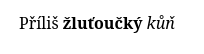
\includegraphics[width=10em]{img/basic.png} 
\end{block}

\end{frame}

V předešlém příkladu \TeX4ht převede LaTeXové příkazy pro tučné a kurzívní písmo na HTML tagy.
Díky tomu, zpracovává DVI soubor, používá informace o použitých fontech a může 
přidat podporu i pro příkazky, které by jinak šly podporovat jen stěží, jako 
\verb|\bfseries| použitý v příkladu.


Pro kompilaci dokumentů pomocí \TeX4ht se používají dva hlavní nástroje: \texttt{make4ht} a \texttt{tex4ebook}.
\texttt{tex4ebook} je starší nástroj, který se používá pro konverzi LaTeXových
dokumentů do formátů pro elektronické knihy, jako je například EPUB.
\texttt{make4ht} vznikl později a je určen pro konverzi LaTeXových dokumentů do
HTML a dalších formátů, jako jsou ODT nebo JATS XML.

\begin{frame}[fragile]{Příklady kompilace pomocí TeX4ht}

\begin{block}{Kompilace do HTML:}
\begin{verbatim}
$ make4ht -ld output_dir soubor.tex
\end{verbatim}
\end{block}



\begin{itemize}
    \item \texttt{-l} - používá Lua\LaTeX\ místo pdf\LaTeX u
    \item \texttt{-d output\_dir} - ukládá výstup do adresáře
\end{itemize}

\begin{block}{Kompilace do EPUB3:}
\begin{verbatim}
$ tex4ebook -f epub3 soubor.tex
\end{verbatim}
\end{block}

\begin{itemize}
    \item \texttt{-f epub3} - specifikuje formát EPUB3
\end{itemize}
\end{frame}

\begin{frame}[fragile]{Konfigurace výstupního formátu}
\begin{block}{Konfigurační soubor pro \TeX4ht}
\begin{verbatim}
\Preamble{xhtml,mathml,mathjax}
\Configure{textit}{\HCode{<i>}\NoFonts}{\EndNoFonts\HCode{</i>}}
\begin{document}
\EndPreamble
\end{verbatim}
\end{block}

\begin{block}{Kompilujeme pomocí:}
\begin{verbatim}
$ make4ht -c config.cfg soubor.tex
\end{verbatim}
\end{block}

\begin{block}{HTML výstup}
\begin{verbatim}
Příliš <span class='cmbx-10'>žluťoučký </span><i>kůň</i>  
\end{verbatim}
\end{block}
\end{frame}

Konfigurační soubor  umožňuje redefinovat výstup
pro příkazy podporované \TeX4ht. V tomto příkladu
se jmenuje \texttt{config.cfg} a voláme ho pomocí volby \texttt{-c}.
Příkaz \verb|\Configure| umožňuje vkládat obsah do háčků, definovaných v 
konfiguračních souborech \TeX4ht pro jednotlivé balíčky. 

V tomto případě využíváme konfiguraci pro \texttt{textit}, která využívá
dva háčky -- jeden vkládá před obsah příkazu \verb|\textit|, druhý za něj.
Tagy vkládáme pomocí příkazu \verb|\HCode|. Abychom zabránili vložení tagů
\verb|<span>| pro aktuální font, použijeme příkaz \verb|\NoFonts|, který 
vypíná zpracování fontů. Na konci konfigurace je třeba opět zpracování fontů
zapnout pomocí \verb|\EndNoFonts|.

\begin{frame}[fragile]{Struktura konfiguračního souboru}
\begin{verbatim}
\Preamble{xhtml,<volby tex4ht>}
<konfigurace>
\begin{document}
<pozdní konfigurace>
\EndPreamble
\end{verbatim}
\end{frame}

Více informací o konfiguračních souborech \TeX4ht naleznete v kapitole
\href{https://www.kodymirus.cz/tex4ht-doc/Configurations.html}{o konfiguracích}
v dokumentaci \TeX4ht.

\begin{frame}[fragile]{Volby pro \TeX4ht}

\begin{block}{}
\begin{verbatim}
$ make4ht soubor.tex "mathml,mathjax"
\end{verbatim}
\begin{itemize}
  \item Volby můžeme zadat jako řetězec v uvozovkách
  \item Další možností je použít příkaz \verb|\Preamble| v konfiguračním souboru
\end{itemize}
\end{block}

\begin{block}{Příklady voleb}
\begin{itemize}
  \item \texttt{mathml} – generuje MathML pro matematické výrazy
  \item \texttt{mathjax} – používá MathJax pro zobrazení matematiky
  \item \texttt{pic-m} - vytváří obrázky pro inline matematiku
  \item \texttt{svg} – generuje SVG obrázky pro TikZ nebo PSTricks
\end{itemize}
\end{block}
\end{frame}

\begin{frame}[fragile]{Rozšíření pro make4ht}
\begin{block}{Povolení rozšíření}
\begin{verbatim}
$ make4ht -f html5+název_rozšíření soubor.tex
\end{verbatim}
\end{block}
\begin{block}{Zakázání rozšíření}
\begin{verbatim}
$ make4ht -f html5-název_rozšíření soubor.tex 
\end{verbatim}
\end{block}



\begin{block}{Příklady rozšíření}
\begin{itemize}
\item \verb|dvisvgm_hashes| -- pro efektivní vytváření SVG obrázků
\item \verb|common_domfilters| -- oprava HTML výstupu pomocí LuaXML
\item \verb|staticsite| -- pro vytvoření souborů ve formátu vhodném pro generátory statických webů
\end{itemize}
\end{block}

\end{frame}

Rozšíření umožňují přizpůsobit chování \TeX4ht pro specifické potřeby. Většinou upravují výstupní soubory
produkované \TeX4ht, například  upravují strukturu HTML dokumentu. 

Rozšíření se povolují nebo zakazují pomocí znamének plus a minus za názvem výstupního formátu. 
Můžeme jich povolit více najednou, například \verb|html5+staticsite+dvisvgm_hashes|.
Některá rozšíření, například \verb|common_domfilters|, jsou povolena implicitně, ale mohou být vypnuta pomocí znaménka minus.

\begin{frame}[fragile]{Build soubory pro TeX4ht}

\begin{block}{Úprava CSS souboru}
\begin{verbatim}
local filter = require("make4ht-filter")  
local process = filter {  
  function(text)  
    -- Nahrazení písma v CSS  
    return text:gsub("TeXGyreTermesX", "Georgia")  
  end  
}  
Make:match("css", process)  -- Aplikuje filtr na CSS soubory
\end{verbatim}
\end{block}

\begin{block}{Použití v make4ht}
\begin{verbatim}
$ make4ht -e build.lua soubor.tex
\end{verbatim}
\end{block}
\end{frame}

Build soubory jsou Lua skripty, které upravují kompilační proces. Například 
v nich můžeme upravovat výstupní soubory. V předešlé ukázce využíváme 
knihovnu \texttt{make4ht-filter} pro úpravu CSS souboru. Pomocí filtru 
můžeme definovat funkce, které upraví text daného souboru. Funkce můžeme řetězit.
V této ukázce nahrazujeme písmo \texttt{TeXGyreTermesX} za \texttt{Georgia} v CSS souboru.
Filtr poté aplikujeme na všechny CSS soubory pomocí příkazu \texttt{Make:match("css", process)}.

\begin{frame}[fragile]{Úprava kompilačního procesu}
\begin{block}{Volání programu Xindex}
\begin{verbatim}
Make:htlatex {} 
Make:xindex {} 
Make:xindex {idxfile = "names.idx"}
Make:autohtlatex {}
\end{verbatim}
\end{block}

\end{frame}

V build souborech můžeme také volat další programy, které se mají spustit. V \texttt{make4ht}
jsou definovány různé funkce, které je spouští. Například \texttt{Make:htlatex} spustí
jednu kompilaci pomocí \LaTeX u, \texttt{Make:xindex} spustí program \texttt{xindex}
a \texttt{Make:autohtlatex} spustí kompilaci \LaTeX em s automatickou detekcí počtu kompilací
nutných k tomu, aby správně fungovaly křížové odkazy nebo tabulky. Ty totiž potřebují více než jednu kompilaci, k tomu
aby se správně vytvořily.

Ve složených závorkách můžeme umístit různé parametry pro daný příkaz. Například 
\verb|Make:xindex {}| bez parametrů zpracuje \texttt{.idx} soubor se stejným základem,
jako je název výstupního souboru. Pokud v dokumentu použijeme více rejstříků, 
například pomocí balíčku \texttt{imakeidx}, můžeme jejich název specifikovat pomocí
parametru \texttt{idxfile}.




% \subsection{GitHub Actions}
\section{Automatické generování HTML výstupu pomocí GitHub Actions}
GitHub, ale i další repozitáře, jako GitLab nebo Bitbucket,  umožňuje
spouštět definované workflow (např. build, testy nebo deploy) v reakci na
události v repozitáři (push, pull request apod.).

Tato funkce se nazývá \href{https://docs.github.com/en/actions/writing-workflows/quickstart}{GitHub Actions} a dále si ukážeme, jak jí využít pro automatizovanou
kompilaci dokumentů pomocí \TeX4ht a jejich publikování na webu.

Šablony pro \TeX4ht, které dále představím, jsou navrženy tak, aby fungovaly v rámci GitHub Actions. To
znamená, že dokumenty mohou být automaticky zkompilovány a publikovány online
pokaždé, když dojde ke změně v repozitáři. Tento přístup zajišťuje, že je
webová verze dokumentu vždy aktuální.


\begin{frame}[fragile]{Příklad worflow souboru}

  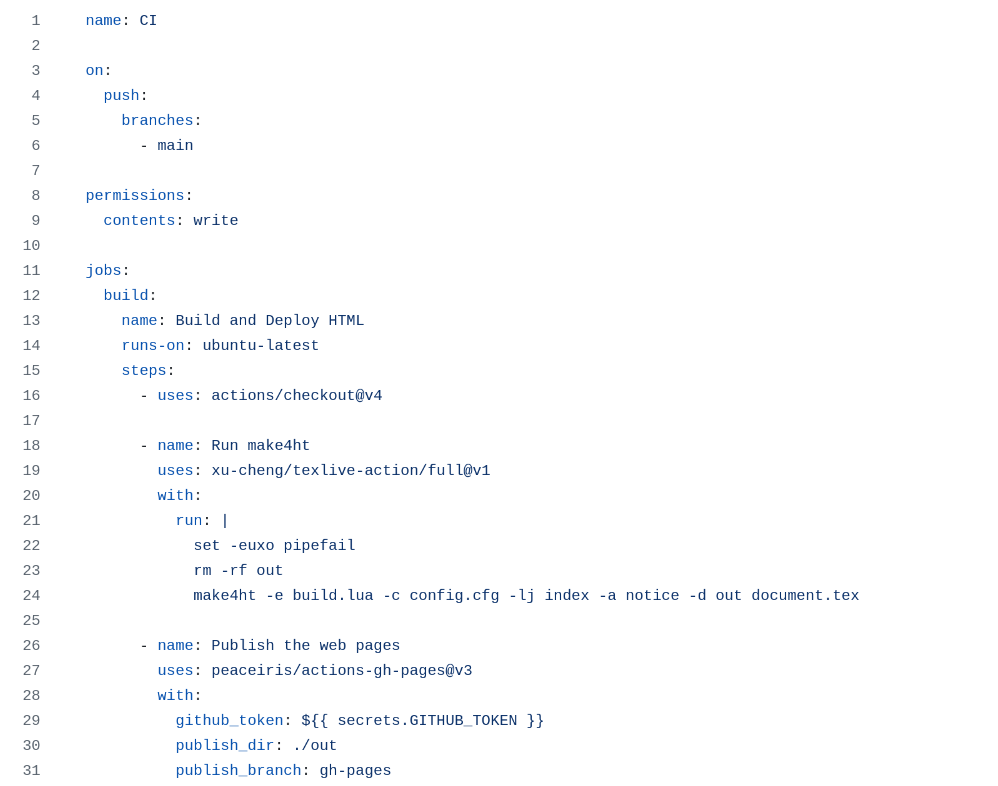
\includegraphics[width=0.7\textwidth]{img/workflow.png}

\end{frame}

Workflow je definován v souboru \texttt{.github/workflows/main.yml}.
Tento soubor můžete upravit pro přizpůsobení procesu sestavení, například změnou parametrů pro \texttt{make4ht}.

\begin{frame}[fragile]{Přehled GitHub Actions}

  \begin{block}{Klíčové části workflow pro sestavení a publikování HTML:}

\begin{verbatim}

  - name: Spuštění make4ht
    uses: xu-cheng/texlive-action/full@v1
    with:
      run: |
        make4ht -lj index -a debug -d out handout.tex

  - name: Publikování webových stránek
    uses: peaceiris/actions-gh-pages@v3
    with:
      github_token: ${{ secrets.GITHUB_TOKEN }}
      publish_dir: ./out
\end{verbatim}
\end{block}

\end{frame}


Používají se dvě GitHub Actions: \href{https://github.com/xu-cheng/texlive-action}{xu-cheng/texlive-action}
a \href{https://github.com/peaceiris/actions-gh-pages}{peaceiris/actions-gh-pages}.
První umožňuje používat libovolný příkaz dostupný v TeX Live instalaci, jako \texttt{make4ht} nebo \texttt{lualatex}.
Druhá publikuje obsah zadaného adresáře do větve \texttt{gh-pages} vašeho repozitáře,
kterou GitHub Pages používá pro zobrazování statického obsahu.

\begin{frame}[fragile]{Automatické sestavení HTML}
\begin{block}{}
Změny pushnuté do větve \texttt{main} spustí GitHub Actions workflow, který:

\begin{itemize}
\item Zkompiluje \texttt{handout.tex} do HTML pomocí \texttt{make4ht}
\item Publikuje výstup do větve \texttt{gh-pages}
\end{itemize}
\end{block}

\begin{block}{Použitý příkaz je:}
\begin{verbatim}
make4ht -lj index -a debug -d out handout.tex
\end{verbatim}
\end{block}
\end{frame}

Tento příkaz vytvoří HTML soubory v adresáři \texttt{out/}, které jsou následně publikovány
pomocí akce \texttt{peaceiris/actions-gh-pages}, specifikované nastavením
\texttt{publish_dir}.

\begin{frame}[fragile]{Proč \texttt{-j index}?}
\begin{itemize}
\item Volba \texttt{-lj index} je zkratka pro \texttt{-l -j index}
\item Volba \texttt{-j index} nastaví název výstupního HTML souboru na \texttt{index.html}
\item To umožňuje používat čisté URL adresy jako:

\begin{verbatim}
https://username.github.io/repo/
\end{verbatim}

\end{itemize}
\end{frame}

Není potřeba v URL specifikovat název souboru - GitHub Pages
automaticky hledá soubor \texttt{index.html}. Toto usnadňuje sdílení
prezentace a pomáhá předejít nefunkčním odkazům kvůli neshodě názvů souborů.



\begin{frame}[fragile]{Rozhraní GitHub Actions}
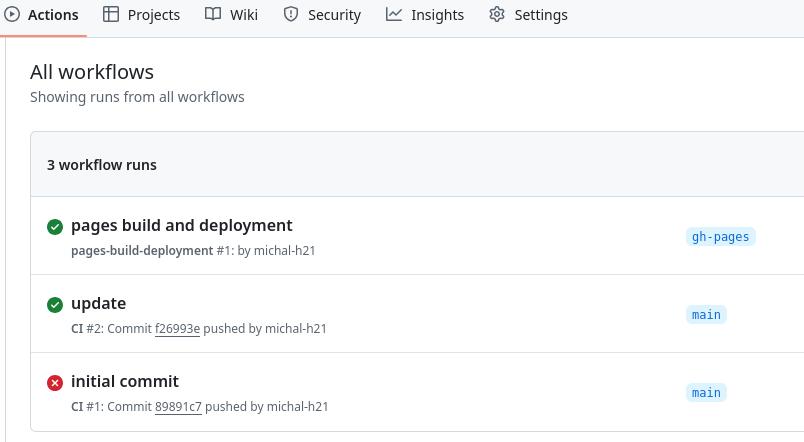
\includegraphics[width=\textwidth]{img/github-actions.png}
\end{frame}

Po každém nahrání změn  můžete zkontrolovat záložku
\texttt{Actions} ve vašem GitHub repozitáři. Zobrazuje stav \textit{workflow}, včetně
informace o úspěšném dokončení nebo případných chybách.

\begin{frame}[fragile]{Chyby}
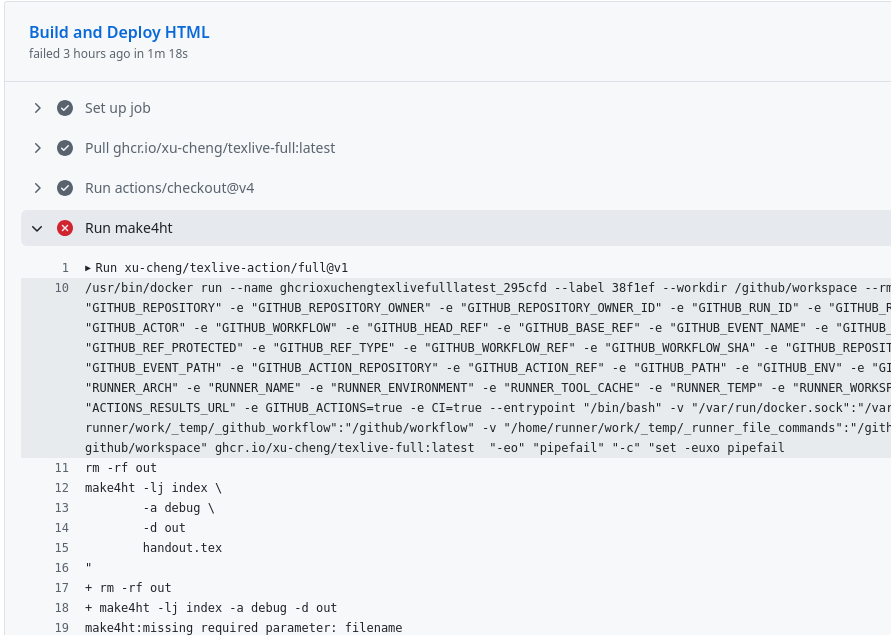
\includegraphics[width=0.75\textwidth]{img/github-error.png}
\end{frame}

Můžete také zkontrolovat logy běhu workflow, abyste viděli, co se pokazilo.
Pokud narazíte na chybu, bude zobrazena v logu a můžete tyto informace
použít k řešení problému.

V tomto případě byl nesprávný název TeX souboru. Musel jsem opravit název
souboru v YAML souboru GitHub Actions.

% \subsection{Publikování HTML verze}

\begin{frame}[fragile]{Nastavení GitHub Pages}
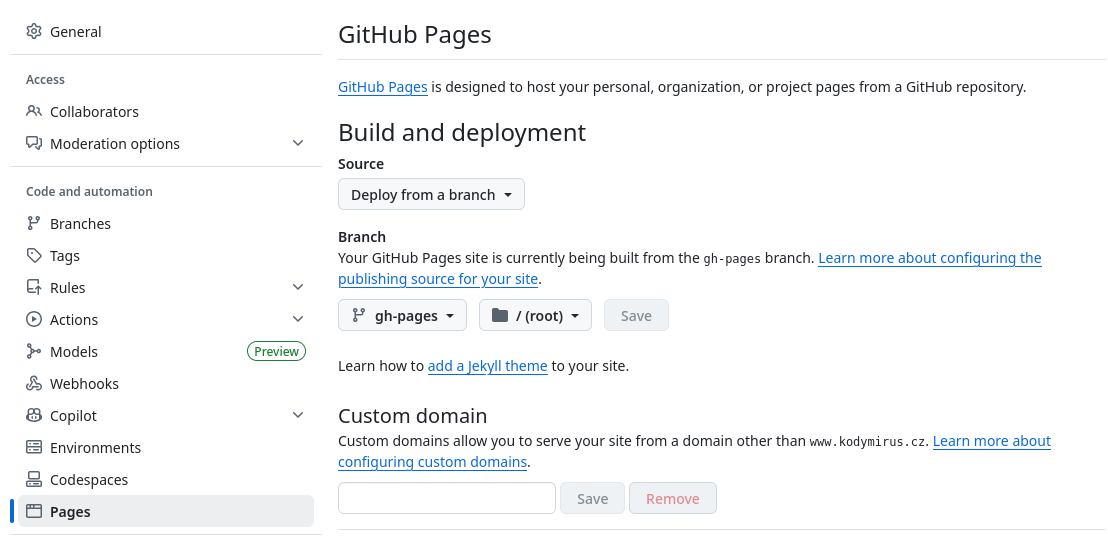
\includegraphics[width=\textwidth]{img/github-pages.png}
\end{frame}

Po úspěšném dokončení workflow můžete nastavit GitHub Pages pro zobrazování obsahu větve \texttt{gh-pages}.

Všechny výstupní soubory vytvořené pomocí \texttt{make4ht} budou dostupné na webu.
Budou přístupné na adrese:
\verb|https://username.github.io/repo/|,
kde \texttt{username} je vaše GitHub uživatelské jméno a \texttt{repo} je název vašeho repozitáře.

Například příklady použité v této prezentaci naleznete na adresách \url{https://michal-h21.github.io/tex4ht-presentation/},
\url{https://michal-h21.github.io/tex4ht-booksite/}

\section{Využití šablon na GitHubu}
\begin{frame}[fragile]{Použití šablony na GitHubu}
  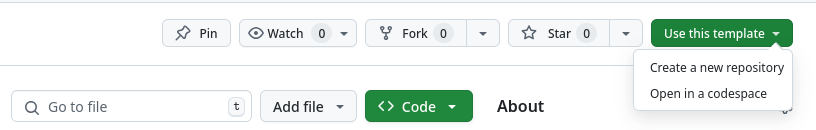
\includegraphics[width=\textwidth,alt={}]{img/template-use.png}
\end{frame}

Pro využití šablon na GitHubu klikněte na tlačítko
\enquote{Use this template} na stránce GitHub repozitáře s podporou šablon. 


\begin{frame}[fragile]{Vytvoření nového GitHub repozitáře}
  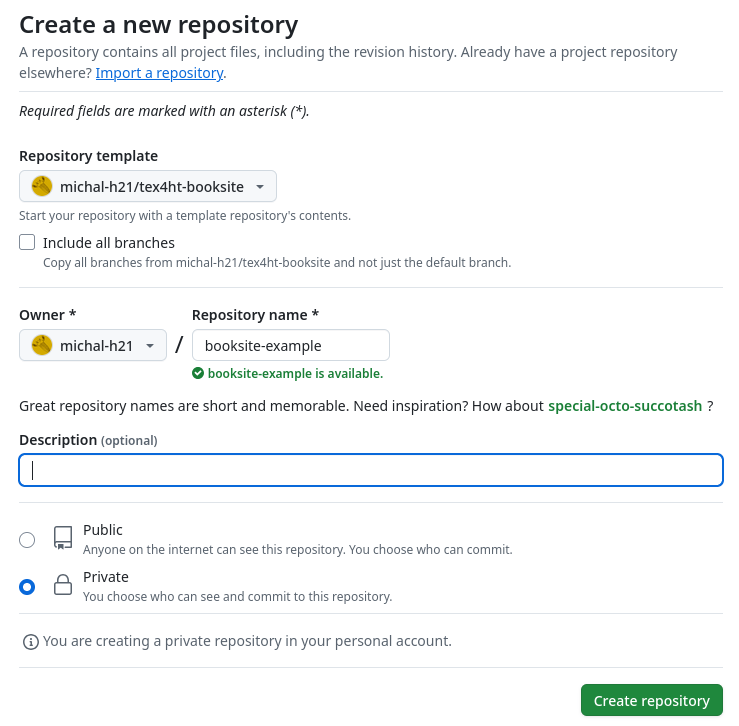
\includegraphics[width=0.6\textwidth,alt={Dialog vytvoření nového repozitáře ze šablony}]{img/new-repo.png}
\end{frame}

Po vyplnění dialogu pro vytvoření nového repozitáře z šablony se ve vašem účtu vytvoří
nový repozitář se stejnou strukturou a soubory, jako měl původní repozitář, ovšem bez jeho 
Git historie.

\begin{frame}[fragile]{Nově vytvořený repozitář}
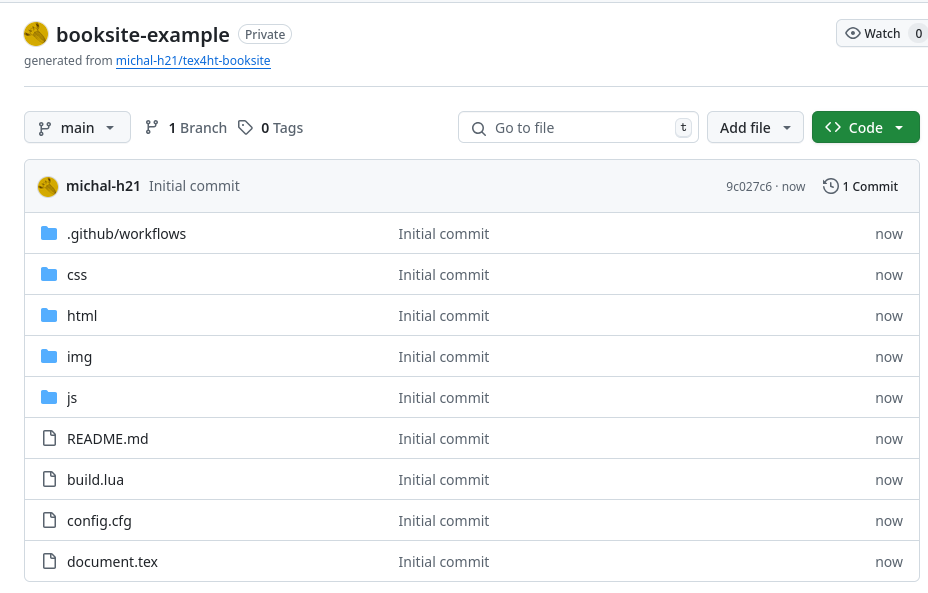
\includegraphics[width=0.6\textwidth]{img/created-repo.png}
\end{frame}


Poté nově vytvořený repozitář můžete naklonovat na svůj počítač a začít upravovat 
obsah souborů. 

\section{Šablona pro webové verze knih}

Tato šablona je navržena tak, aby umožňovala export každé kapitoly do
samostatné HTML stránky. Je ideální pro publikaci knihy, dokumentace nebo
skript, kde každá kapitola tvoří vlastní webovou stránku propojenou navigací.

\begin{frame}[fragile]{Export kapitol na samostané stránky}
\begin{block}{}
\begin{verbatim}
$ make4ht document.tex "2"
\end{verbatim}
\end{block}

\begin{figure}
  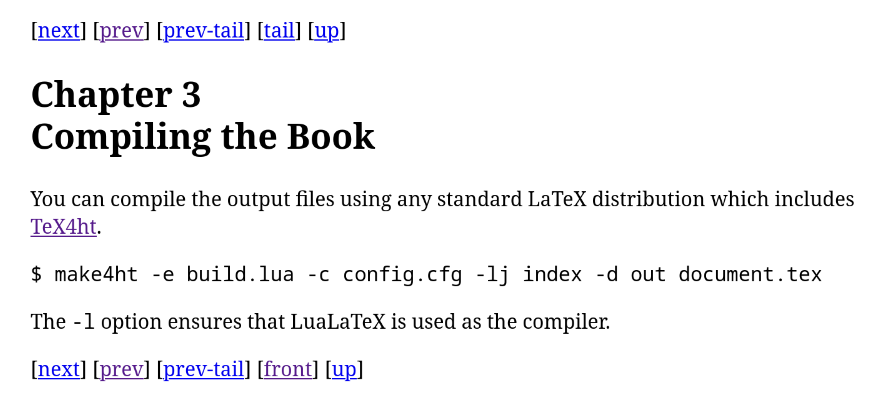
\includegraphics[width=0.8\textwidth]{img/plain-chapter.png}
\end{figure}
\end{frame}

Číselné volby umožňují nastavit, od které úrovně členění textu se mají vytvářet
samostatné soubory. Například volba s hodnotou 1 způsobí, že budou vytvořeny
samostatné soubory pro nejvyšší úroveň struktury dokumentu. Hodnota 2 zajistí
rozdělení i pro další úroveň, obvykle kapitoly, případně sekce, pokud typ
dokumentu kapitoly neobsahuje. Při volbě 3 se soubory vytvářejí i pro sekce, a
to i u typů dokumentů, které běžně kapitoly obsahují. Takto lze pokračovat až
do úrovně 7, kdy jsou samostatné soubory generovány i pro velmi jemné členění,
na úrovní příkazů \verb|\paragraph|.

Obecně doporučuji použít volbu "2".

Ve výchozí podobě jednotlivé soubory kapitol obsahují jen základní navigaci,
s odkazy na předchozí a následující kapitolu a na hlavní soubor.

\begin{frame}[fragile]{Názvy souborů}
\begin{block}{Defaultně se vytváří názvy souboru ve formě:}
\begin{verbatim}
název souboru + úroveň nadpisu + pořadí
\end{verbatim}
\end{block}

\begin{block}{Například:}
\begin{verbatim}
document.html
documentch1.html
documentch2.html
documentch3.html
documentli1.html
\end{verbatim}
\end{block}
\end{frame}

V prvním souboru se nachází obsah, který se v dokumentu objevil před první kapitolou, například obsah příkazu 
\verb|\maketitle|. Dále obsahuje obsah s odkazy na jednotlivé kapitoly. Soubor s koncovkou \verb|li| se vytváří 
pro nečíslované kapitoly, například rejstřík nebo seznam literatury.

Problém je, když změníme pořadí kapitol nebo přidáme novou kapitolu. Odkazy dovnitř kapitol mohou přestat fungovat.

\begin{frame}[fragile]{Pojmenování souborů}
  \begin{block}{Mějme kapitolu v češtině}
    \begin{verbatim}
\chapter{Kapitola s háčky}
    \end{verbatim}
  \end{block}

  \begin{block}{Základní volba pro pojmenování kapitol na základě jejich názvu}
  \begin{verbatim}
$ make4ht document.tex "2,sec-filename"
Kapitolasháčky.html
    \end{verbatim}
  \end{block}
\begin{block}{Alternativa pro čistější názvy:}
\begin{verbatim}
$ make4ht -l document.tex "2,sec-slugname"
kapitola_s_hacky.html
\end{verbatim}
\end{block}

\end{frame}

Volba \verb|sec-slugname| produkuje názvy souborů, které jsou lépe využitelné
na webu. Veškerou diakritiku nahradí za ASCII znaky, převede velká písmena na
malá, odstraní znaky které nejsou písmena a mezery nahradí podtržítky. Pro svou
funkcionalitu ovšem vyžaduje přepínač \verb|-l|, protože název se vytváří
pomocí Lua.

\begin{frame}[fragile]{Boční menu}

\begin{block}{}
\begin{verbatim}
$ make4ht document.tex "2,sec-slugname,fulltoc"
\end{verbatim}
\end{block}

\begin{figure}
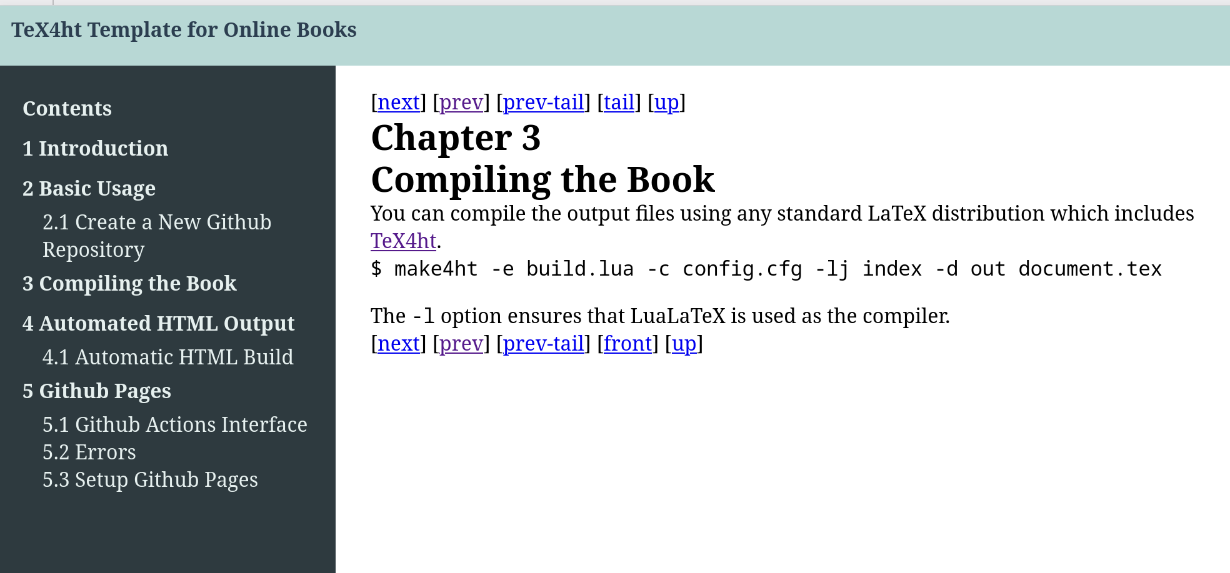
\includegraphics[width=0.8\textwidth]{img/fulltoc-basic.png}
\end{figure}

\end{frame}

Volba "fulltoc" vytvoří na každé stránce boční menu obsahující plný obsah knihy. 
Díky tomu lze snadno přecházet mezi jednotlivými kapitolami. Ovšem toto menu 
může být poměrně rozsáhlé, pokud je v knize hodně podkapitol. Můžeme chtít 
zobrazit jen sekce aktuální kapitoly a podsekce ostatních kapitol skrýt. 
Pro to můžeme využít build soubor pro \texttt{make4ht} a DOM filtr 
\texttt{collapsetoc}. Další možností je využití JavaScriptu.

Obě tyto možnosti jsou zpřístupněné v následující šabloně.

\begin{frame}[fragile]{Šablona \texttt{tex4ht-booksite}}

\begin{block}{Adresa:}
\url{https://github.com/michal-h21/tex4ht-booksite}
\end{block}

\begin{block}{Hlavní vlastnosti}
  \begin{itemize}
    \item Zobrazuje pouze sekce aktuální kapitoly
    \item Automaticky zobrazuje a skrývá hlavičku a patičku stránky
    \item Skrývá menu na malých obrazovkách
  \end{itemize}
\end{block}

\end{frame}

\begin{frame}[fragile]{Zobrazí pouze aktuální podsekce}

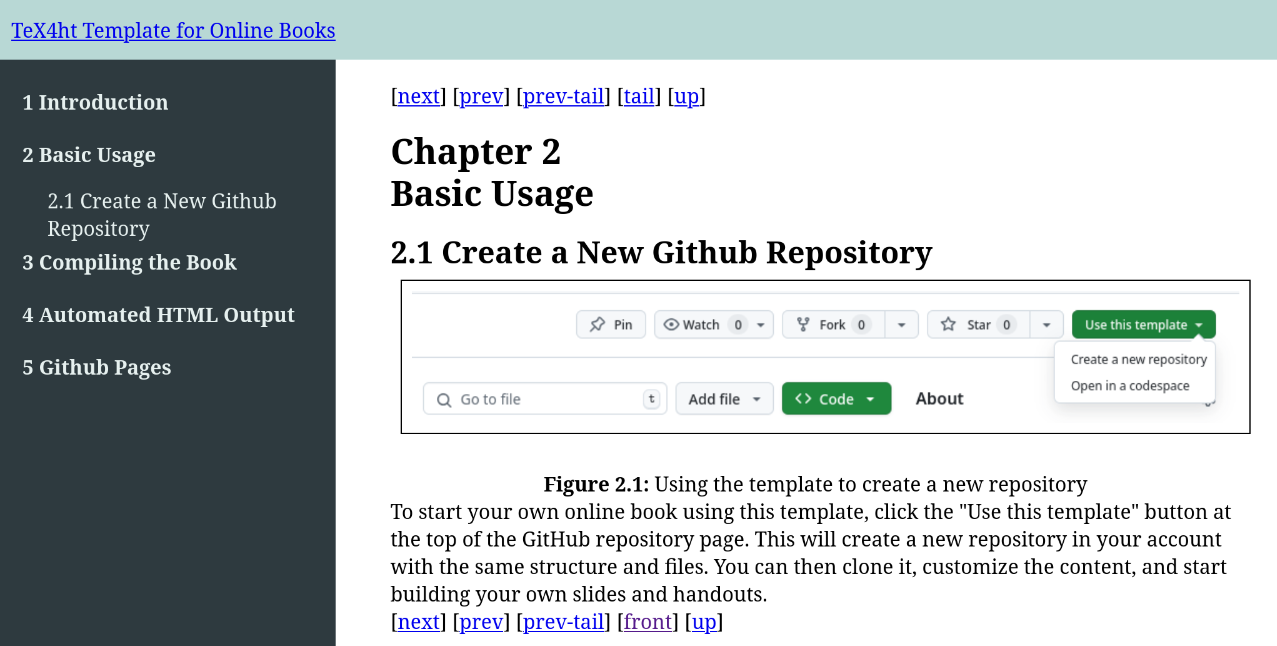
\includegraphics[width=0.8\textwidth]{img/collapsetoc.png}

\end{frame}

\begin{frame}{Skrytí menu na malých displejích}
 \begin{columns}
    \begin{column}{0.48\textwidth}
      \begin{block}{Skryté menu}
      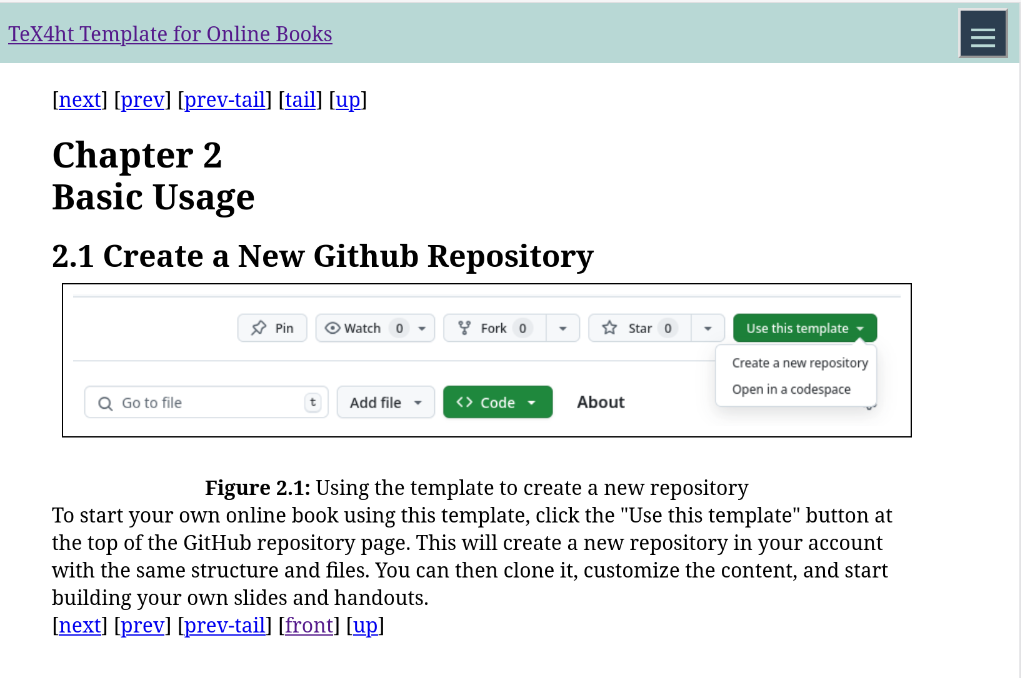
\includegraphics[width=\linewidth]{img/book-hamburger.png}
    \end{block}
    \end{column}
    \begin{column}{0.48\textwidth}
      \begin{block}{Otevřené menu}
      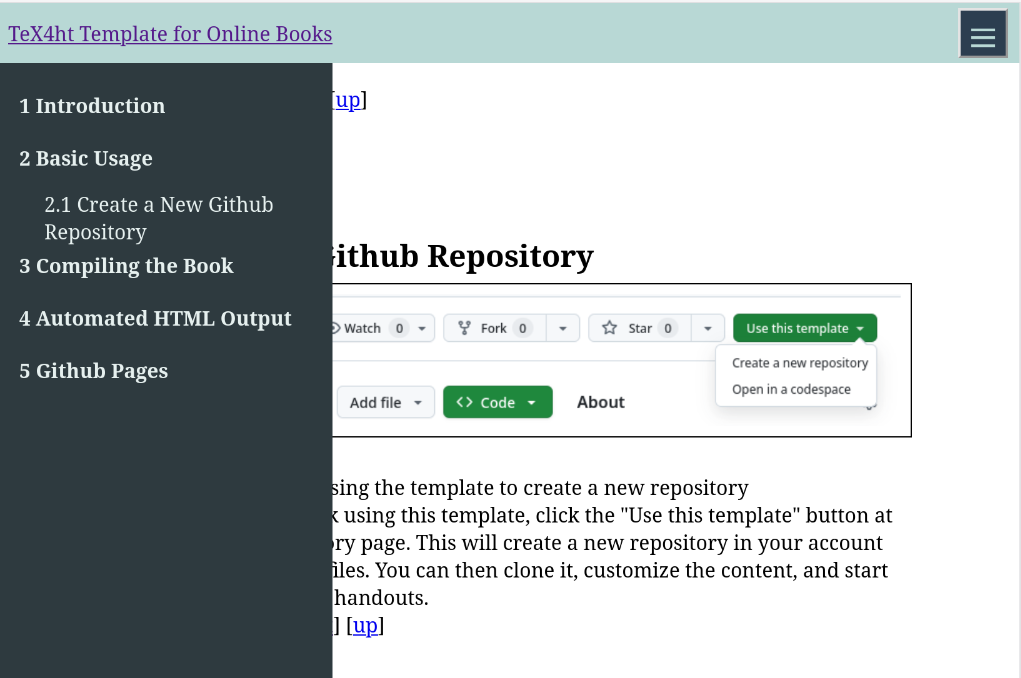
\includegraphics[width=\linewidth]{img/book-hamburger-open.png}
    \end{block}
    \end{column}
  \end{columns}
\end{frame}

Skrytí menu je užitečné především na mobilních zařízeních s menším displejem, kde by při 
zobrazeném menu nezůstalo dostatek místa pro zobrazení samotného textu dokumentu.
Pro zobrazení menu využíváme JavaScript, kterému se jinak snažím vyhýbat. 

Většina barev v šabloně je nastavená pomocí CSS proměnných, které můžeme změnit v konfiguračním souboru.

\begin{frame}[fragile]{Podporované vlastnosti pro změnu designu stránky}
  \begin{block}{}
    \begin{description}
      \item[maintoc] -- menu s obsahem dokumentu
      \item[hamburger] -- tlačítko pro schované menu
      \item[header] -- hlavička dokumentu
      \item[footer] -- patička dokumentu
    \end{description}
  \end{block}
  \begin{block}{}
    Pro každou z těchto vlastností můžete nastavit barvu popředí a pozadí přidáním \texttt{-color} a \texttt{-background} 
    k jejich názvu.
  \end{block}

\end{frame}

\begin{frame}[fragile]{Změna barev}

  \begin{block}{Přidejte do konfiguračního souboru \texttt{config.cfg}}
\begin{verbatim}
\Css{
  body{
    --maintoc-background: \#f0f0f0;
    --maintoc-color: \#00AFA0;
  }
}
\end{verbatim}
\end{block}

\begin{block}{Boční menu se změněnými barvami}
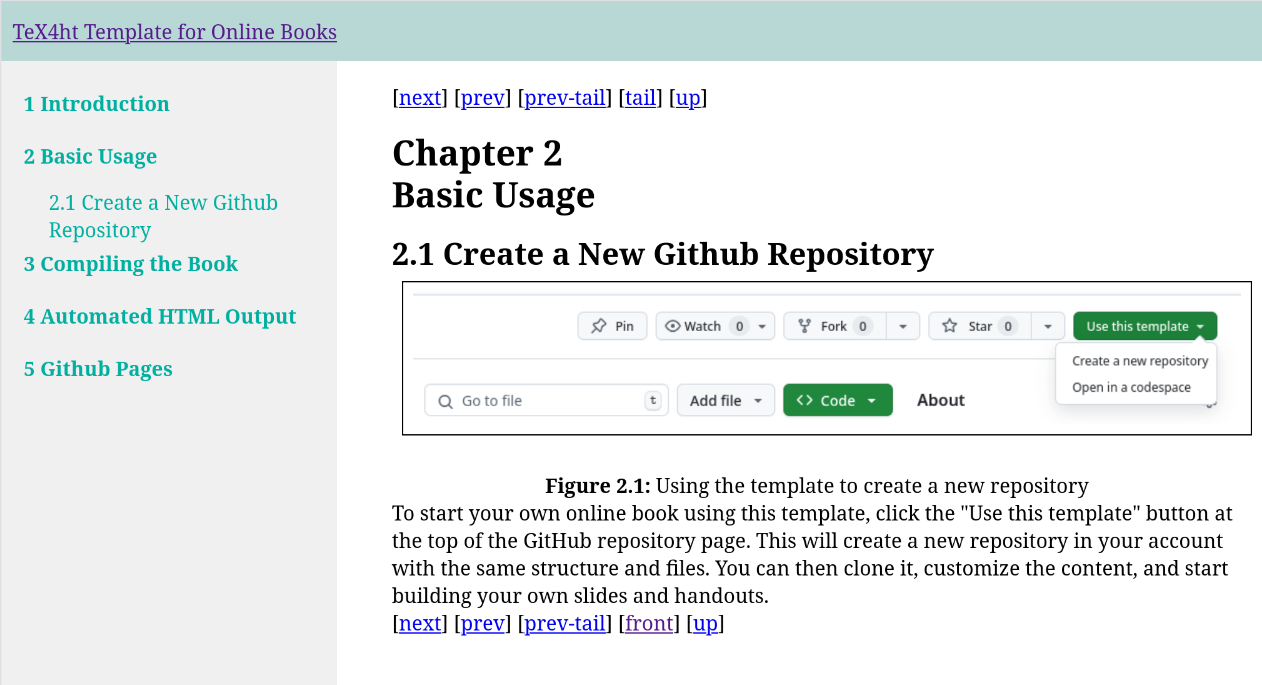
\includegraphics[width=0.8\textwidth]{img/book-changecolor.png}
\end{block}
\end{frame}


Příkaz \verb|\Css| můžete vložit do konfiguračního souboru \texttt{config.cfg} 
kamkoliv mezi \verb|\Preamble| a \verb|\EndPreamble|. Při použití hexadecimálního 
zápisu je třeba escapovat znak \verb|#| pomocí zpětného lomítka, jinak dojde ke
kompilační chybě.

Konfigurační soubor obsahuje mnoho dalších možností nastavení, ale rozsah naší prezentace
nám neumožňuje všechny představit. Zároveň na této šabloně stále aktivně pracuji, takže 
je pravděpodobné, že se bude dále měnit. Sledujte tedy prosím její
\href{https://www.kodymirus.cz/tex4ht-booksite/}{dokumentaci}.

\section{Šablona pro blogy}

\begin{frame}[fragile]{Jak můžeme blogovat s \LaTeX em?}


\begin{itemize}
\item Blogování s využitím generátorů statických webů
\item Každý článek je samostatný \TeX ový dokument v samostatném adresáři
\item Automatická kompilace změněných článků
\end{itemize}

\end{frame}


\begin{frame}[fragile]{Co je statický generátor webu?}

  \begin{block}{Hlavní vlastnosti}
  \begin{itemize}
    \item ze vstupních souborů kompiluje webové stránky, například blogy
    \item soubory se generují pouze při aktualizaci webu
    \item většinou aplikují šablony na zdrojové soubory
    \item vytváří seznamy článků, RSS a podobně
    \item můžeme je spouštět v prostředí GitHub Actions
    \item GitHub obsahuje vestavěný generátor Jekyll
  \end{itemize}
\end{block}
\end{frame}

Výhodou je, že takový web můžeme umístit na téměř libovolný webový server,
nemusíme řešit, zda podporuje například PHP nebo jiný systém pro dynamické 
zobrazování stránek. Například GitHub nabízí GitHub Pages, kde můžeme 
umístit stránky zdarma. V rámci GitHub Actions také můžeme spouštět generátory
automaticky, nebo můžeme využít vestavěnou podporu pro generátor Jekyll.


\begin{frame}[fragile]{Obecná struktura vstupního souboru}

\begin{block}{Příklad pro Markdown}
\begin{verbatim}
---
title: Titulek dokumentu
---
# Úvod
Text dokumentu
\end{verbatim}
\end{block}

\end{frame}

Na začátku souboru je umístěný blok s metadaty dokumentu ve formátu YAML. Z obou stran
je obklopený řádky obsahujícími pouze tři spojovníky. Za blokem metadat pak následuje 
text dokumentu.

V tomto příkladě používáme Markdown, ovšem stejný princip 
můžeme použít i pro HTML soubory produkované pomocí \TeX4ht.
Místo Markdownu totiž můžeme použít i HTML, které získáme z obsahu elementu 
\verb|<body>|

\begin{frame}[fragile]{Ukázka s \TeX4ht}
\begin{block}{\LaTeX ový dokument:}
\begin{verbatim}

\documentclass{article}
\begin{document}
\title{Hello world test}
\author{Michal}
\maketitle

This is my test post.
\end{document}
\end{verbatim}
\end{block}

\begin{block}{Kompilujeme pomocí}
\begin{verbatim}
$ make4ht -f html5+staticsite filename.tex
\end{verbatim}
\end{block}
\end{frame}

V tomto případě musíme zapnout rozšíření \texttt{staticsite}, které jsme připojili za formát souboru 
ve volbě \texttt{-f}. Toto rozšíření vytvoří HTML soubor ve formátu vhodném pro statické generátory.
Soubor bude pojmenován ve formátu \verb|YYYY-MM-DD-<filename>|. 

\begin{frame}[fragile]{Vygenerovaný soubor}
  \begin{verbatim}
---
meta:
- charset: ’utf-8’
- name: ’viewport’
  content: ’width=device-width,initial-scale=1’
time: 1626619562
updated: 1627244699
styles:
- ’2021-07-18-hello-world.css’
title: ’Hello world test’
---
<!--  l. 7  --><p class=’indent’>   This is my test post.
</p>
  \end{verbatim}
\end{frame}

Soubor obsahuje různá metadata získaná z HTML souboru. Jednak se jedná 
o obsah elementů \verb|<meta>|, dále časy vytvoření souboru a poslední aktualizace v číselné formě, 
seznam použitých stylů, titulek atd. Tato metadata můžeme používat v šablonách 
použitého generátoru webů.



\begin{frame}[fragile]{Šablona pro blog s generátorem Jekyll}

\begin{block}{Adresa:}
\url{https://github.com/michal-h21/testblog/}
\end{block}

\begin{block}{Ukázka hlavní stránky blogu}
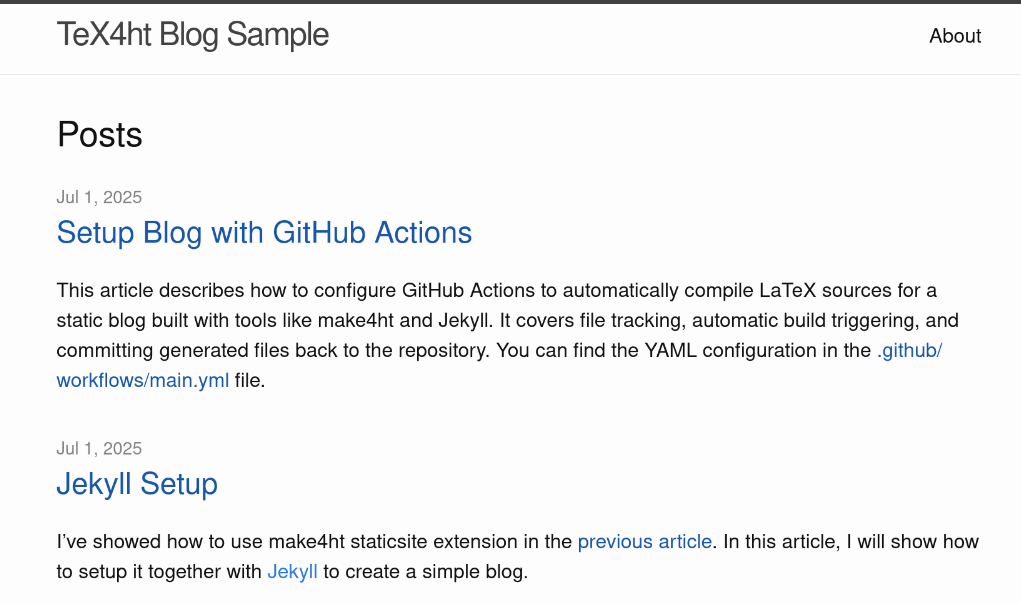
\includegraphics[width=0.6\textwidth]{img/blog.png}
\end{block}

\end{frame}

\begin{frame}[fragile]{Struktura adresářů}
\begin{verbatim}
blog/
.. texposts/
.... first_post/
...... first_post.tex
.... second_post/
...... second_post.tex
.. docs/
.... _posts/
.... css
\end{verbatim}
\end{frame}

Každý příspěvek na blogu má vlastní podadresář v adrsáři \texttt{texposts}. 
Vygenerované soubory se poté zkopírují do různých podadresářů v adresáři 
\texttt{docs}. Například HTML soubory pro blog se umístí do podadresáře 
\verb|_posts| a kaskádové style do podadresáře \texttt{css}.

\begin{frame}[fragile]{Postup zpracování v šabloně}
\begin{itemize}
\item detekujeme změněné \TeX ové soubory a zkompilujeme je
\item zkopírujeme vygenerované soubory do adresářů, kde je bude hledat Jekyll
\item vygenerované soubory uložíme do repozitáře
\item poté je zpracuje statický generátor Jekyll, který vytvoří blog
\end{itemize}
\end{frame}

Vygenerované soubory ukládáme proto, abychom v příštích kompilacích 
mohli porovnat datumy změn HTML a \TeX\ souborů. Kompilujeme poté pouze soubory, 
které nemají vygenerovaný HTML soubor, nebo je tento soubor starší.
Tím zrychlujeme kompilaci a šetříme výpočetní čas GitHub Actions. 

Tento projekt je poměrně komplikovaný a stále funguje spíše jako 
ukázka funkčnosti. Stále se mi nepodařilo vyřešit některé problémy 
s konflikty lokálních a vzdálených verzí souborů. Přesto si myslím, 
že může být zajímavé jej představit. Doufám, že aktuální problémy se 
mi brzy podaří vyřešit.



\section{Šablona pro prezentace}

Tato šablona je určena pro prezentace, které potřebují víc než jen snímky.
Umožňuje vytvořit jak samotnou prezentaci, tak podrobný handout s poznámkami a
komentáři. Všechny materiály tak lze generovat z jednoho zdrojového souboru –
jak pro živou prezentaci, tak pro lidi, kteří se prezentace neúčastnili.

\begin{frame}[fragile]{Šablona \texttt{tex4ht-presentation}}

\begin{block}{Adresa:}
\url{https://github.com/michal-h21/tex4ht-presentation}
\end{block}

\begin{block}{Hlavní vlastnosti}
  \begin{itemize}
    \item Vytváří slidy a handout prezentací ze stejného zdrojového souboru
  \end{itemize}
\end{block}

\end{frame}

\begin{frame}[fragile]{Co je cílem?}
\begin{block}{HTML handout}
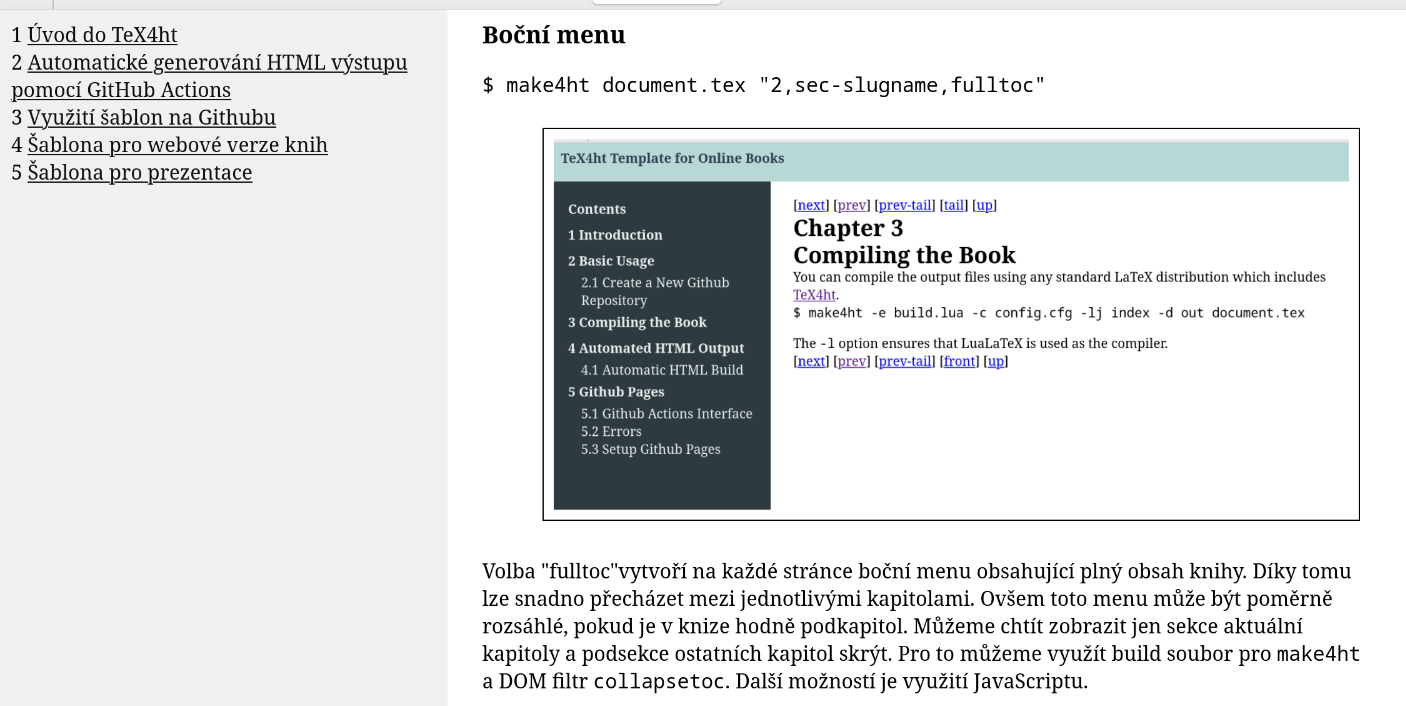
\includegraphics[width=0.8\textwidth]{img/handout.png}
\end{block}

\end{frame}


Šablona obshuje několik hlavních zdrojových souborů, každý s konkrétním účelem:

\begin{frame}[fragile]{Přehled souborů}
\begin{block}{Soubory ke kompilaci}
\begin{itemize}
\item \textbf{\texttt{slides.tex}}
\item \textbf{\texttt{handout.tex}}
\end{itemize}
\end{block}
\begin{block}{Text prezentace}
\begin{itemize}
\item \textbf{\texttt{presentation.tex}}
\end{itemize}
\end{block}
\begin{block}{Konfigurační soubory}
\begin{itemize}
\item \textbf{\texttt{preamble.tex}}
\item \textbf{\texttt{config.cfg}}
\end{itemize}
\end{block}
\end{frame}

% \bigskip
% \noindent\textbf{Popis souborů}
\paragraph{Popis souborů}
% \medskip
\begin{itemize}

\item \textbf{\texttt{slides.tex}} – Tento soubor slouží ke generování hlavní prezentace ve formátu Beamer. Obsahuje to, co se zobrazuje během přednášky.

\item \textbf{\texttt{handout.tex}} – Handoutová verze prezentace, formátovaná
  jako standardní článek. Kromě obsahu viditelného na snímcích obsahuje i
  doplňující poznámky a komentáře, které se v samotné prezentaci nezobrazují.
  Tento soubor je určen ke sdílení po skončení prezentace a měl by být
  samostatně použitelný i pro čtenáře, kteří prezentaci neviděli.

\item \textbf{\texttt{presentation.tex}} – Obsahuje celý zdrojový text
  prezentace. Obsah uvnitř prostředí
  \verb|\begin|\verb|{frame}...\end|\verb|{frame}| se zahrnuje jak do
  \texttt{slides.tex}, tak do \texttt{handout.tex}. Text mimo prostředí frame
  se v prezentaci nezobrazí, ale je součástí handoutu. To umožňuje doplnit
  prezentaci o podrobnější komentáře, vysvětlení nebo poznámky.

\item \textbf{preamble.tex} – Obsahuje balíčky a definice příkazů používané v prezentaci.

\item \textbf{config.cfg} – Konfigurační soubor pro \TeX4ht. Například zde můžete upravit CSS styly použité ve webové verzi dokumentu nebo redefinice \LaTeX{}ových příkazů.
\end{itemize}

\begin{frame}[fragile]{Hlavní soubor pro slidy}
\begin{verbatim}
\documentclass[ignorenonframetext]{beamer}
\usepackage{hyperref}
\usepackage{graphicx}
\usepackage[czech]{babel}
\usepackage{csquotes}
\usepackage{luavlna}
% I use this environment to force linebreaks one source code listing
% that doesn't work well with TeX4ht otherwise. It is redefined in config.cfg. 
% you can remove it if you don't need it.
\newenvironment{likeverbatim}{}{}
 % sdílené nastavení preamble
\begin{document}
\mode<beamer>{
  % if you want to include some content outside of frames also in slides, use \mode<
\mode<beamer|article>{
  \title{Publikace LaTeXových dokumentů na web pomocí TeX4ht a GitHub Actions}
  \author{Michal Hoftich}
  \maketitle
}

\begin{abstract}
Přednáška představí sadu šablon pro nástroj TeX4ht, který slouží k převodu
LaTeXových dokumentů do HTML. Tyto šablony výrazně usnadňují publikaci různých
typů dokumentů na webu a přinášejí moderní možnosti zpracování a automatizace.

První šablona je určena pro převod knižních dokumentů do webové podoby.
Umožňuje rozdělení textu do jednotlivých kapitol s automaticky generovanou
navigací a podporou responzivního designu, takže je výsledek dobře čitelný i na
mobilních zařízeních.

Druhá šablona slouží k tvorbě staticky generovaných blogů. Každý příspěvek je
psán jako samostatný LaTeXový dokument, který je pomocí TeX4ht převeden do
HTML. Následně jsou tyto články zpracovány statickým generátorem webů, jako je
například Jekyll, který se postará o sestavení celého blogu, vytvoření
rozcestníků, archivů a další navigace.

Třetí šablona je zaměřena na převod prezentací vytvořených v prostředí Beamer
do formy tzv. handoutů – přehledových materiálů pro posluchače. Výsledkem je
čitelný a dobře strukturovaný webový dokument vhodný pro sdílení po přednášce.

Všechny šablony jsou navrženy tak, aby fungovaly v rámci GitHub Actions. To
znamená, že dokumenty mohou být automaticky zkompilovány a publikovány online
pokaždé, když dojde ke změně v repozitáři. Tento přístup zajišťuje, že je
webová verze dokumentu vždy aktuální.
\end{abstract}


\tableofcontents

\section{Úvod do TeX4ht}

\begin{frame}{Co je TeX4ht?}
\begin{itemize}
    \item \textbf{Nástroj pro konverzi} z LaTeXu do HTML a dalších formátů (ODT, EPUB, JATS XML)
    \item Zachovává strukturu a formátování původního dokumentu
    \item Podporuje různé metody pro matematický výstup (obrázky, MathML, MathJax)
    \item Umožňuje vytvářet obrázky z výstupu \LaTeX u
    \item Integruje se s běžnými LaTeXovými balíčky
\end{itemize}
\end{frame}

\TeX4ht samotný je především balíček, který redefinuje příkazy jiných balíčků tak, aby
vkládaly tagy výstupních formátů. Vždy se kompiluje do DVI výstupu, který se poté zpracovává
dalšími nástroji, které vytvoří soubory ve výstupním formátu, CSS soubor, nebo obrázky.
Části DVI výstupu lze konvertovat na obrázky ve formátu PNG nebo SVG. To se využívá pro podporu
TikZ nebo PSTricks.

Více informací o \TeX4ht naleznete na  \href{https://www.tug.org/tex4ht/}{oficiálních stránkách}
a v \href{https://www.kodymirus.cz/tex4ht-doc/tex4ht-doc.html}{dokumentaci}.

\begin{frame}[fragile]{Příklad použití TeX4ht}


\begin{block}{Příklad LaTeX kódu}
\begin{verbatim}
Příliš {\bfseries žluťoučký} \textit{kůň}
\end{verbatim}
\end{block}



\begin{block}{Výstup v HTML kódu}
\begin{verbatim}
Příliš <span class='cmbx-10'>žluťoučký </span>
<span class='cmti-10'>kůň</span>
\end{verbatim}
\end{block}

\begin{block}{Výstup v prohlížeči}
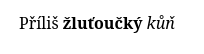
\includegraphics{img/basic.png} 
\end{block}

\end{frame}

V předešlém příkladu \TeX4ht převede LaTeXové příkazy pro tučné a kurzívní písmo na HTML tagy.
Díky tomu, zpracovává DVI soubor, používá informace o použitých fontech a může 
přidat podporu i pro příkazky, které by jinak šly podporovat jen stěží, jako 
\verb|\bfseries| použitý v příkladu.


Pro kompilaci dokumentů pomocí \TeX4ht se používají dva hlavní nástroje: \texttt{make4ht} a \texttt{tex4ebook}.
\texttt{tex4ebook} je starší nástroj, který se používá pro konverzi LaTeXových
dokumentů do formátů pro elektronické knihy, jako je například EPUB.
\texttt{make4ht} vznikl později a je určen pro konverzi LaTeXových dokumentů do
HTML a dalších formátů, jako jsou ODT nebo JATS XML.

\begin{frame}[fragile]{Příklady kompilace pomocí TeX4ht}

\begin{block}{Kompilace do HTML:}
\begin{verbatim}
$ make4ht -ld output_dir soubor.tex
\end{verbatim}
\end{block}



\begin{itemize}
    \item \texttt{-l} - používá Lua\LaTeX\ místo pdf\LaTeX u
    \item \texttt{-d output\_dir} - ukládá výstup do adresáře
\end{itemize}

\begin{block}{Kompilace do EPUB3:}
\begin{verbatim}
$ tex4ebook -f epub3 soubor.tex
\end{verbatim}
\end{block}

\begin{itemize}
    \item \texttt{-f epub3} - specifikuje formát EPUB3
\end{itemize}
\end{frame}

\begin{frame}[fragile]{Konfigurace výstupního formátu}
\begin{block}{Konfigurační soubor pro \TeX4ht}
\begin{verbatim}
\Preamble{xhtml}
\Configure{textit}{\HCode{<i>}\NoFonts}{\EndNoFonts\HCode{</i>}}
\begin{document}
\EndPreamble
\end{verbatim}
\end{block}

\begin{block}{Kompilujeme pomocí:}
\begin{verbatim}
$ make4ht -c config.cfg soubor.tex
\end{verbatim}
\end{block}

\begin{block}{HTML výstup}
\begin{verbatim}
Příliš <span class='cmbx-10'>žluťoučký </span><i>kůň</i>  
\end{verbatim}
\end{block}
\end{frame}

Konfigurační soubor  umožňuje redefinovat výstup
pro příkazy podporované \TeX4ht. V tomto příkladu
se jmenuje \texttt{config.cfg} a voláme ho pomocí volby \texttt{-c}.
Příkaz \verb|\Configure| umožňuje vkládat obsah do háčků, definovaných v 
konfiguračních souborech \TeX4ht pro jednotlivé balíčky. 

V tomto případě využíváme konfiguraci pro \texttt{textit}, která využívá
dva háčky -- jeden vkládá před obsah příkazu \verb|\textit|, druhý za něj.
Tagy vkládáme pomocí příkazu \verb|\HCode|. Abychom zabránili vložení tagů
\verb|<span>| pro aktuální font, použijeme příkaz \verb|\NoFonts|, který 
vypíná zpracování fontů. Na konci konfigurace je třeba opět zpracování fontů
zapnout pomocí \verb|\EndNoFonts|.

\begin{frame}[fragile]{Struktura konfiguračního souboru}
\begin{verbatim}
\Preamble{xhtml,<volby tex4ht>}
<konfigurace>
\begin{document}
<pozdní konfigurace>
\EndPreamble
\end{verbatim}
\end{frame}

Více informací o konfiguračních souborech \TeX4ht naleznete v kapitole
\href{https://www.kodymirus.cz/tex4ht-doc/Configurations.html}{o konfiguracích}
v dokumentaci \TeX4ht.

\begin{frame}[fragile]{Volby pro \TeX4ht}

\begin{block}{}
\begin{verbatim}
$ make4ht soubor.tex "mathml,mathjax"
\end{verbatim}
\begin{itemize}
  \item Volby můžeme zadat jako řetězec v uvozovkách
  \item Další možností je použít příkaz \verb|\Preamble| v konfiguračním souboru
\end{itemize}
\end{block}

\begin{block}{Příklady voleb}
\begin{itemize}
  \item \texttt{mathml} – generuje MathML pro matematické výrazy
  \item \texttt{mathjax} – používá MathJax pro zobrazení matematiky
  \item \texttt{pic-m} - vytváří obrázky pro inline matematiku
  \item \texttt{svg} – generuje SVG obrázky pro TikZ nebo PSTricks
\end{itemize}
\end{block}
\end{frame}

\begin{frame}[fragile]{Rozšíření pro make4ht}
\begin{block}{Povolení rozšíření}
\begin{verbatim}
$ make4ht -f html5+název_rozšíření soubor.tex
\end{verbatim}
\end{block}
\begin{block}{Zakázání rozšíření}
\begin{verbatim}
$ make4ht -f html5-název_rozšíření soubor.tex 
\end{verbatim}
\end{block}



\begin{block}{Příklady rozšíření}
\begin{itemize}
\item \verb|dvisvgm_hashes| -- pro efektivní vytváření SVG obrázků
\item \verb|common_domfilters| -- oprava HTML výstupu pomocí LuaXML
\item \verb|staticsite| -- pro vytvoření souborů ve formátu vhodném pro generátory statických webů
\end{itemize}
\end{block}

\end{frame}

Rozšíření umožňují přizpůsobit chování \TeX4ht pro specifické potřeby. Většinou upravují výstupní soubory
produkované \TeX4ht, například  upravují strukturu HTML dokumentu. 

Rozšíření se povolují nebo zakazují pomocí znamének plus a minus za názvem výstupního formátu. 
Můžeme jich povolit více najednou, například \verb|html5+staticsite+dvisvgm_hashes|.
Některá rozšíření, například \verb|common_domfilters|, jsou povolena implicitně, ale mohou být vypnuta pomocí znaménka minus.

\begin{frame}[fragile]{Build soubory pro TeX4ht}

\begin{block}{Úprava CSS souboru}
\begin{verbatim}
local filter = require("make4ht-filter")  
local process = filter {  
  function(text)  
    -- Nahrazení písma v CSS  
    return text:gsub("TeXGyreTermesX", "Georgia")  
  end  
}  
Make:match("css", process)  -- Aplikuje filtr na CSS soubory
\end{verbatim}
\end{block}

\begin{block}{Použití v make4ht}
\begin{verbatim}
$ make4ht -e build.lua soubor.tex
\end{verbatim}
\end{block}
\end{frame}

Build soubory jsou Lua skripty, které upravují kompilační proces. Například 
v nich můžeme upravovat výstupní soubory. V předešlé ukázce využíváme 
knihovnu \texttt{make4ht-filter} pro úpravu CSS souboru. Pomocí filtru 
můžeme definovat funkce, které upraví text daného souboru. Funkce můžeme řetězit.
V této ukázce nahrazujeme písmo \texttt{TeXGyreTermesX} za \texttt{Georgia} v CSS souboru.
Filtr poté aplikujeme na všechny CSS soubory pomocí příkazu \texttt{Make:match("css", process)}.

\begin{frame}[fragile]{Úprava kompilačního procesu}
\begin{block}{Volání programu Xindex}
\begin{verbatim}
Make:htlatex {} 
Make:xindex {} 
Make:autohtlatex {}
\end{verbatim}
\end{block}

\end{frame}

V build souborech můžeme také volat další programy, které se mají spustit. V \texttt{make4ht}
jsou definovány různé funkce, které je spouští. Například \texttt{Make:htlatex} spustí
jednu kompilaci pomocí \LaTeX u, \texttt{Make:xindex} spustí program \texttt{xindex}
a \texttt{Make:autohtlatex} spustí kompilaci \LaTeX em s automatickou detekcí počtu kompilací
nutných k tomu, aby správně fungovaly křížové odkazy nebo tabulky. Ty totiž potřebují více než jednu kompilaci, k tomu
aby se správně vytvořily.


\section{Využití Githubu pro automatické publikování}

\begin{frame}[fragile]{Použití šablony na GitHubu}
  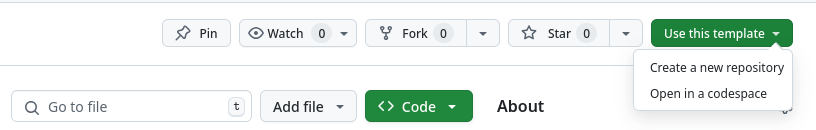
\includegraphics[width=\textwidth,alt={}]{img/template-use.png}
\end{frame}

Pro využití šablon na Githubu klikněte na tlačítko
\enquote{Use this template} na stránce GitHub repozitáře s podporou šablon. 

Tím se ve vašem účtu vytvoří
nový repozitář se stejnou strukturou a soubory. Poté jej můžete naklonovat,
upravit obsah a začít vytvářet vlastní snímky a handouty.

\begin{frame}[fragile]{Vytvoření nového GitHub repozitáře}
  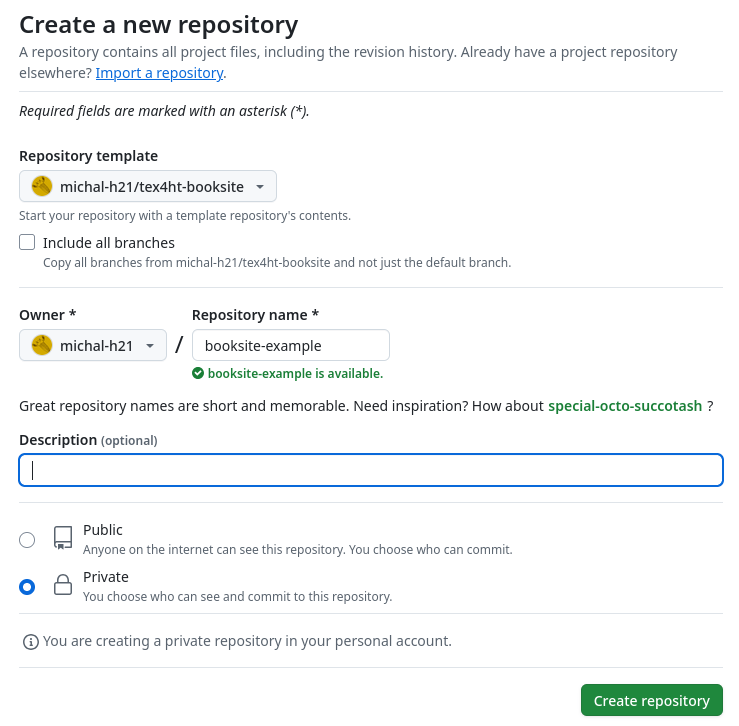
\includegraphics[width=0.6\textwidth,alt={Dialog vytvoření nového repozitáře ze šablony}]{img/new-repo.png}
\end{frame}

Po 

% \subsection{Github Actions}

\begin{frame}[fragile]{Rozhraní Github Actions}
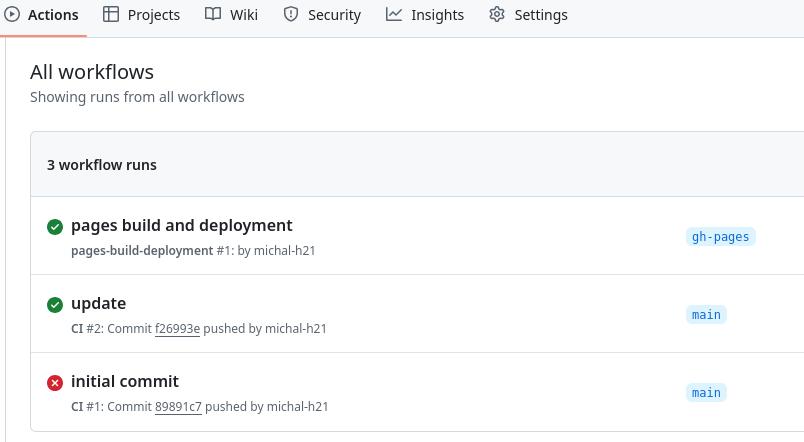
\includegraphics[width=\textwidth]{img/github-actions.png}
\end{frame}

Po pushnutí změn do větve \texttt{main} můžete zkontrolovat záložku
\texttt{Actions} ve vašem Github repozitáři. Zobrazuje stav workflow, včetně
informace o úspěšném dokončení nebo případných chybách.

\begin{frame}[fragile]{Chyby}
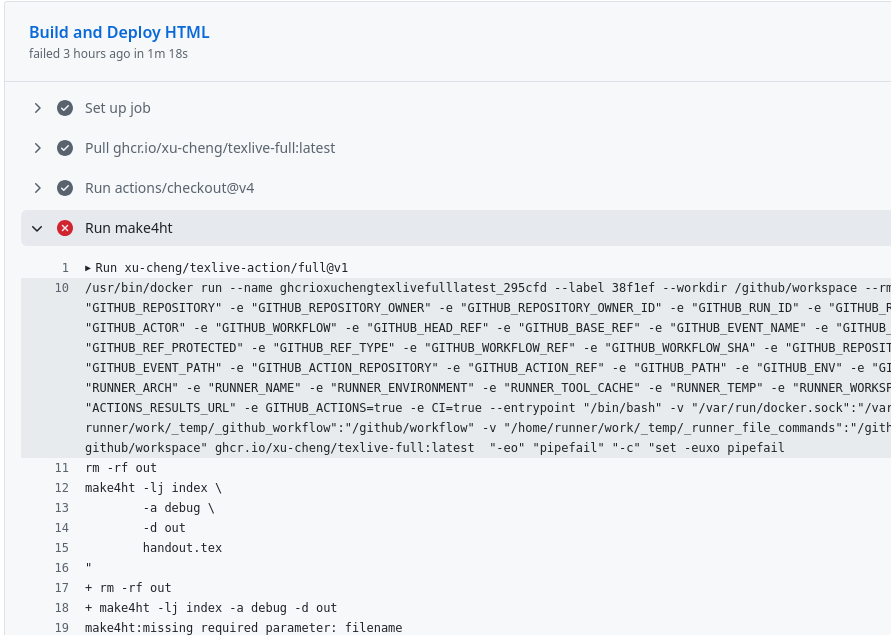
\includegraphics[width=\textwidth]{img/github-error.png}
\end{frame}

Můžete také zkontrolovat logy běhu workflow, abyste viděli, co se pokazilo.
Pokud narazíte na chybu, bude zobrazena v logu a můžete tyto informace
použít k řešení problému.

V tomto případě byl nesprávný název TeX souboru. Musel jsem opravit název
souboru v YAML souboru GitHub Actions.

% \subsection{Publikování HTML verze}

\begin{frame}[fragile]{Nastavení Github Pages}
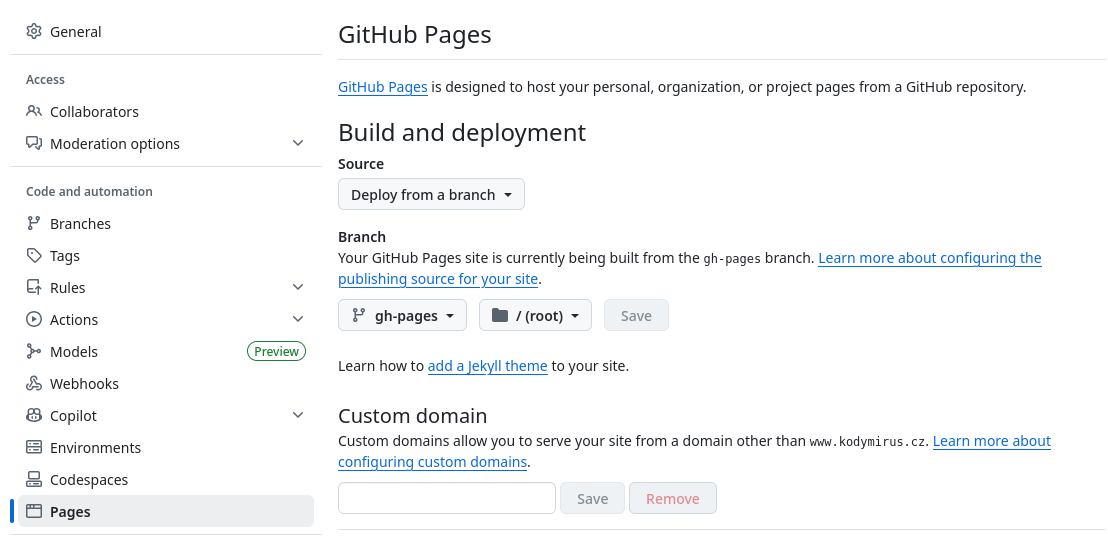
\includegraphics[width=\textwidth]{img/github-pages.png}
\end{frame}

Po úspěšném dokončení workflow můžete nastavit GitHub Pages pro zobrazování obsahu větve \texttt{gh-pages}.

Všechny výstupní soubory vytvořené pomocí \texttt{make4ht} budou dostupné na webu.
Budou přístupné na adrese:
\verb|https://username.github.io/repo/|,
kde \texttt{username} je vaše GitHub uživatelské jméno a \texttt{repo} je název vašeho repozitáře.

Například příklady použité v této prezentaci naleznete na adresách \url{https://michal-h21.github.io/tex4ht-presentation/},
\url{https://michal-h21.github.io/tex4ht-booksite/}

\section{Šablona pro prezentace}

Tato šablona je určena pro prezentace, které potřebují víc než jen snímky. Umožňuje vytvořit jak samotnou prezentaci, tak podrobný handout s poznámkami a komentáři. Všechny materiály tak lze generovat z jednoho zdrojového souboru – jak pro živou prezentaci, tak pro lidi, kteří se prezentace neúčastnili.

Obsahuje několik hlavních zdrojových souborů, každý s konkrétním účelem:

\begin{frame}[fragile]{Přehled souborů}
\begin{itemize}
\item \textbf{\texttt{slides.tex}}
\item \textbf{\texttt{handout.tex}}
\item \textbf{\texttt{presentation.tex}}
\item \textbf{\texttt{preamble.tex}}
\item \textbf{\texttt{config.cfg}}
\end{itemize}
\end{frame}

\begin{itemize}
\item \textbf{\texttt{slides.tex}} – Tento soubor slouží ke generování hlavní prezentace ve formátu Beamer. Obsahuje to, co se zobrazuje během přednášky.

\item \textbf{\texttt{handout.tex}} – Handoutová verze prezentace, formátovaná jako standardní článek. Kromě obsahu viditelného na snímcích obsahuje i doplňující poznámky a komentáře, které se v samotné prezentaci nezobrazují. Tento soubor je určen ke sdílení po skončení prezentace a měl by být samostatně použitelný i pro čtenáře, kteří prezentaci neviděli.

\item \textbf{\texttt{presentation.tex}} – Obsahuje celý zdrojový text prezentace. Obsah uvnitř prostředí \verb|\begin{frame}...\end{frame}| se zahrnuje jak do \texttt{slides.tex}, tak do \texttt{handout.tex}. Text mimo prostředí frame se v prezentaci nezobrazí, ale je součástí handoutu. To umožňuje doplnit prezentaci o podrobnější komentáře, vysvětlení nebo poznámky.

\item \textbf{preamble.tex} – Obsahuje balíčky a definice příkazů používané v prezentaci.

\item \textbf{config.cfg} – Konfigurační soubor pro \TeX4ht. Například zde můžete upravit CSS styly použité ve webové verzi dokumentu nebo redefinice \LaTeX{}ových příkazů.
\end{itemize}

Tyto soubory si můžete upravit podle svých potřeb. Minimálně je vhodné nahradit obsah \texttt{presentation.tex} vlastním textem a případně upravit \texttt{preamble.tex}, pokud potřebujete přidat další balíčky nebo příkazy.

\subsection{Základní použití}


\begin{frame}[fragile]{Použití prostředí frame a komentáře v handoutu}

\begin{block}{}
Základní syntaxe dokumentu používaného v souboru \verb|presentation.tex| vypadá následovně:
\end{block}

\begin{likeverbatim}\verb|\begin{frame}{Název snímku}|\
\verb|obsah snímku...|\
\verb|\end|\verb|{frame}|\
\vspace{1em}
\verb|Komentář, který bude zahrnut pouze v handoutu|
\end{likeverbatim}

\end{frame}

Například zdrojový kód jednoho z předchozích snímků vypadá takto:

\verb|\begin|\verb|{frame}[fragile]{Přehled souborů}|
\begin{verbatim}
\begin{itemize}
\item \textbf{\texttt{slides.tex}}
\item \textbf{\texttt{handout.tex}}
\item \textbf{\texttt{presentation.tex}}
\item \textbf{\texttt{preamble.tex}}
\end{itemize}
\end{verbatim}
\verb|\end|\verb|{frame}|

\begin{verbatim}
\begin{itemize}
\item \textbf{\texttt{slides.tex}} – Tento soubor slouží ke generování hlavní
prezentace ve formátu Beamer. Obsahuje to, co se zobrazuje během přednášky.
\end{itemize}
\end{verbatim}

Obsah uvnitř bloku \verb|\begin|\verb|{frame}...\end|\verb|{frame}| se zahrne
do prezentace i handoutu, ale prostředí \texttt{itemize}, které následuje za
ním, se zobrazí pouze v handoutu.

\begin{frame}[fragile]{Sdílený obsah mimo prostředí frame}

\begin{verbatim}
\mode<beamer|article>{
\title{Strukturovaná šablona prezentace}
\author{Michal Hoftich}
\maketitle
}
\end{verbatim}
\end{frame}

Příkaz \verb+\mode<beamer|article>{...}+ umožňuje zahrnout obsah, který se má
zobrazit jak v prezentaci, tak v handoutu. To se může hodit například pro název
prezentace nebo obsah prezentace.

\subsection{Kompilace prezentace}

\begin{frame}[fragile]{Kompilace do PDF}

Prezentaci nebo handout můžete zkompilovat do PDF pomocí LuaLaTeXu těmito příkazy:

\begin{verbatim}
$ lualatex slides.tex
$ lualatex handout.tex
\end{verbatim}
\end{frame}



Výstupní soubory můžete kompilovat v libovolné standardní distribuci \LaTeX{}u, která obsahuje Beamer a potřebné balíčky.

\begin{frame}[fragile]{HTML verze}
Pro převod prezentace do formátu HTML použijte nástroj \href{https://www.tug.org/tex4ht/}{\TeX4ht}.
\begin{verbatim}
$ make4ht -l handout.tex\end{verbatim}

Přepínač \verb|-l| zajistí použití Lua\LaTeX{}u jako překladače.
\end{frame}

HTML verze se generuje z handoutu ve stylu článku, nikoliv z Beamer prezentace.
To ji činí vhodnější pro webové publikování nebo dlouhodobé sdílení, protože
obsahuje všechny vysvětlivky a není závislá na rozvržení snímků.

section{Automatické generování HTML výstupu}

Tato část vysvětluje, jak se používají \href{https://docs.github.com/en/actions/writing-workflows/quickstart}{GitHub Actions} k automatickému generování a publikování HTML verze materiálů při každém pushnutí změn do větve \texttt{main}.

Výstup je vytvářen pomocí \texttt{make4ht} a publikován do větve \texttt{gh-pages}, což usnadňuje sdílení webové verze prezentace.

\begin{frame}[fragile]{Přehled GitHub Actions}
Klíčové části workflow pro sestavení a publikování HTML:

\begin{verbatim}

    name: Spuštění make4ht
    uses: xu-cheng/texlive-action/full@v1
    with:
      run: |
      make4ht -lj index -a debug -d out handout.tex

    name: Publikování webových stránek
    uses: peaceiris/actions-gh-pages@v3
    with:
      github_token: ${{ secrets.GITHUB_TOKEN }}
      publish_dir: ./out
\end{verbatim}

\end{frame}

Workflow je definován v souboru \texttt{.github/workflows/main.yml}.
Tento soubor můžete upravit pro přizpůsobení procesu sestavení, například změnou parametrů pro \texttt{make4ht}.

Používají se dvě GitHub Actions: \href{https://github.com/xu-cheng/texlive-action}{xu-cheng/texlive-action}
a \href{https://github.com/peaceiris/actions-gh-pages}{peaceiris/actions-gh-pages}.
První umožňuje používat libovolný příkaz dostupný v TeX Live instalaci, jako \texttt{make4ht} nebo \texttt{lualatex}.
Druhá publikuje obsah zadaného adresáře do větve \texttt{gh-pages} vašeho repozitáře,
kterou GitHub Pages používá pro zobrazování statického obsahu.

\begin{frame}[fragile]{Automatické sestavení HTML}
Změny pushnuté do větve \texttt{main} spustí GitHub Actions workflow, který:

\begin{itemize}
\item Zkompiluje \texttt{handout.tex} do HTML pomocí \texttt{make4ht}
\item Publikuje výstup do větve \texttt{gh-pages}
\end{itemize}

Použitý příkaz je:

\begin{verbatim}
make4ht -lj index -a debug -d out handout.tex
\end{verbatim}
\end{frame}

Tento příkaz vytvoří HTML soubory v adresáři \texttt{out/}, které jsou následně publikovány
pomocí akce \texttt{peaceiris/actions-gh-pages}, specifikované nastavením
\texttt{publish_dir}.

\begin{frame}[fragile]{Proč \texttt{-j index}?}
\begin{itemize}
\item Volba \texttt{-lj index} je zkratka pro \texttt{-l -j index}
\item Volba \texttt{-j index} nastaví název výstupního HTML souboru na \texttt{index.html}
\item To umožňuje používat čisté URL adresy jako:

\begin{verbatim}
https://username.github.io/repo/
\end{verbatim}

\end{itemize}
\end{frame}

Není potřeba v URL specifikovat název souboru - GitHub Pages
automaticky hledá soubor \texttt{index.html}. Toto usnadňuje sdílení
prezentace a pomáhá předejít nefunkčním odkazům kvůli neshodě názvů souborů.



}
\end{document}
\end{verbatim}
\end{frame}

Volba \texttt{ignorenonframetext} má za následek, že veškerý text mimo prostředí \texttt{frame} se ignoruje.
Díky tomu můžeme psát komentáře mimo slidy, které se zobrazí pouze v handoutu. Problém je, že se ignoruje i příkaz
\verb|\input|, který používáme pro vložení textu prezentace z externího souboru. Musíme proto použít příkaz 
\verb|\|\verb|mode|, který umí lokálně přepnout mód. Pro vložení obsahu do prezentace využijeme mód \verb|<beamer>|.

\begin{frame}[fragile]{Hlavní soubor pro handout}
\begin{verbatim}
\documentclass{article}
\usepackage{beamerarticle}
\usepackage{hyperref}
\usepackage{graphicx}
\usepackage[czech]{babel}
\usepackage{csquotes}
\usepackage{luavlna}
% I use this environment to force linebreaks one source code listing
% that doesn't work well with TeX4ht otherwise. It is redefined in config.cfg. 
% you can remove it if you don't need it.
\newenvironment{likeverbatim}{}{}

\begin{document}
% if you want to include some content outside of frames also in slides, use \mode<
\mode<beamer|article>{
  \title{Publikace LaTeXových dokumentů na web pomocí TeX4ht a GitHub Actions}
  \author{Michal Hoftich}
  \maketitle
}

\begin{abstract}
Přednáška představí sadu šablon pro nástroj TeX4ht, který slouží k převodu
LaTeXových dokumentů do HTML. Tyto šablony výrazně usnadňují publikaci různých
typů dokumentů na webu a přinášejí moderní možnosti zpracování a automatizace.

První šablona je určena pro převod knižních dokumentů do webové podoby.
Umožňuje rozdělení textu do jednotlivých kapitol s automaticky generovanou
navigací a podporou responzivního designu, takže je výsledek dobře čitelný i na
mobilních zařízeních.

Druhá šablona slouží k tvorbě staticky generovaných blogů. Každý příspěvek je
psán jako samostatný LaTeXový dokument, který je pomocí TeX4ht převeden do
HTML. Následně jsou tyto články zpracovány statickým generátorem webů, jako je
například Jekyll, který se postará o sestavení celého blogu, vytvoření
rozcestníků, archivů a další navigace.

Třetí šablona je zaměřena na převod prezentací vytvořených v prostředí Beamer
do formy tzv. handoutů – přehledových materiálů pro posluchače. Výsledkem je
čitelný a dobře strukturovaný webový dokument vhodný pro sdílení po přednášce.

Všechny šablony jsou navrženy tak, aby fungovaly v rámci GitHub Actions. To
znamená, že dokumenty mohou být automaticky zkompilovány a publikovány online
pokaždé, když dojde ke změně v repozitáři. Tento přístup zajišťuje, že je
webová verze dokumentu vždy aktuální.
\end{abstract}


\tableofcontents

\section{Úvod do TeX4ht}

\begin{frame}{Co je TeX4ht?}
\begin{itemize}
    \item \textbf{Nástroj pro konverzi} z LaTeXu do HTML a dalších formátů (ODT, EPUB, JATS XML)
    \item Zachovává strukturu a formátování původního dokumentu
    \item Podporuje různé metody pro matematický výstup (obrázky, MathML, MathJax)
    \item Umožňuje vytvářet obrázky z výstupu \LaTeX u
    \item Integruje se s běžnými LaTeXovými balíčky
\end{itemize}
\end{frame}

\TeX4ht samotný je především balíček, který redefinuje příkazy jiných balíčků tak, aby
vkládaly tagy výstupních formátů. Vždy se kompiluje do DVI výstupu, který se poté zpracovává
dalšími nástroji, které vytvoří soubory ve výstupním formátu, CSS soubor, nebo obrázky.
Části DVI výstupu lze konvertovat na obrázky ve formátu PNG nebo SVG. To se využívá pro podporu
TikZ nebo PSTricks.

Více informací o \TeX4ht naleznete na  \href{https://www.tug.org/tex4ht/}{oficiálních stránkách}
a v \href{https://www.kodymirus.cz/tex4ht-doc/tex4ht-doc.html}{dokumentaci}.

\begin{frame}[fragile]{Příklad použití TeX4ht}


\begin{block}{Příklad LaTeX kódu}
\begin{verbatim}
Příliš {\bfseries žluťoučký} \textit{kůň}
\end{verbatim}
\end{block}



\begin{block}{Výstup v HTML kódu}
\begin{verbatim}
Příliš <span class='cmbx-10'>žluťoučký </span>
<span class='cmti-10'>kůň</span>
\end{verbatim}
\end{block}

\begin{block}{Výstup v prohlížeči}
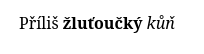
\includegraphics{img/basic.png} 
\end{block}

\end{frame}

V předešlém příkladu \TeX4ht převede LaTeXové příkazy pro tučné a kurzívní písmo na HTML tagy.
Díky tomu, zpracovává DVI soubor, používá informace o použitých fontech a může 
přidat podporu i pro příkazky, které by jinak šly podporovat jen stěží, jako 
\verb|\bfseries| použitý v příkladu.


Pro kompilaci dokumentů pomocí \TeX4ht se používají dva hlavní nástroje: \texttt{make4ht} a \texttt{tex4ebook}.
\texttt{tex4ebook} je starší nástroj, který se používá pro konverzi LaTeXových
dokumentů do formátů pro elektronické knihy, jako je například EPUB.
\texttt{make4ht} vznikl později a je určen pro konverzi LaTeXových dokumentů do
HTML a dalších formátů, jako jsou ODT nebo JATS XML.

\begin{frame}[fragile]{Příklady kompilace pomocí TeX4ht}

\begin{block}{Kompilace do HTML:}
\begin{verbatim}
$ make4ht -ld output_dir soubor.tex
\end{verbatim}
\end{block}



\begin{itemize}
    \item \texttt{-l} - používá Lua\LaTeX\ místo pdf\LaTeX u
    \item \texttt{-d output\_dir} - ukládá výstup do adresáře
\end{itemize}

\begin{block}{Kompilace do EPUB3:}
\begin{verbatim}
$ tex4ebook -f epub3 soubor.tex
\end{verbatim}
\end{block}

\begin{itemize}
    \item \texttt{-f epub3} - specifikuje formát EPUB3
\end{itemize}
\end{frame}

\begin{frame}[fragile]{Konfigurace výstupního formátu}
\begin{block}{Konfigurační soubor pro \TeX4ht}
\begin{verbatim}
\Preamble{xhtml}
\Configure{textit}{\HCode{<i>}\NoFonts}{\EndNoFonts\HCode{</i>}}
\begin{document}
\EndPreamble
\end{verbatim}
\end{block}

\begin{block}{Kompilujeme pomocí:}
\begin{verbatim}
$ make4ht -c config.cfg soubor.tex
\end{verbatim}
\end{block}

\begin{block}{HTML výstup}
\begin{verbatim}
Příliš <span class='cmbx-10'>žluťoučký </span><i>kůň</i>  
\end{verbatim}
\end{block}
\end{frame}

Konfigurační soubor  umožňuje redefinovat výstup
pro příkazy podporované \TeX4ht. V tomto příkladu
se jmenuje \texttt{config.cfg} a voláme ho pomocí volby \texttt{-c}.
Příkaz \verb|\Configure| umožňuje vkládat obsah do háčků, definovaných v 
konfiguračních souborech \TeX4ht pro jednotlivé balíčky. 

V tomto případě využíváme konfiguraci pro \texttt{textit}, která využívá
dva háčky -- jeden vkládá před obsah příkazu \verb|\textit|, druhý za něj.
Tagy vkládáme pomocí příkazu \verb|\HCode|. Abychom zabránili vložení tagů
\verb|<span>| pro aktuální font, použijeme příkaz \verb|\NoFonts|, který 
vypíná zpracování fontů. Na konci konfigurace je třeba opět zpracování fontů
zapnout pomocí \verb|\EndNoFonts|.

\begin{frame}[fragile]{Struktura konfiguračního souboru}
\begin{verbatim}
\Preamble{xhtml,<volby tex4ht>}
<konfigurace>
\begin{document}
<pozdní konfigurace>
\EndPreamble
\end{verbatim}
\end{frame}

Více informací o konfiguračních souborech \TeX4ht naleznete v kapitole
\href{https://www.kodymirus.cz/tex4ht-doc/Configurations.html}{o konfiguracích}
v dokumentaci \TeX4ht.

\begin{frame}[fragile]{Volby pro \TeX4ht}

\begin{block}{}
\begin{verbatim}
$ make4ht soubor.tex "mathml,mathjax"
\end{verbatim}
\begin{itemize}
  \item Volby můžeme zadat jako řetězec v uvozovkách
  \item Další možností je použít příkaz \verb|\Preamble| v konfiguračním souboru
\end{itemize}
\end{block}

\begin{block}{Příklady voleb}
\begin{itemize}
  \item \texttt{mathml} – generuje MathML pro matematické výrazy
  \item \texttt{mathjax} – používá MathJax pro zobrazení matematiky
  \item \texttt{pic-m} - vytváří obrázky pro inline matematiku
  \item \texttt{svg} – generuje SVG obrázky pro TikZ nebo PSTricks
\end{itemize}
\end{block}
\end{frame}

\begin{frame}[fragile]{Rozšíření pro make4ht}
\begin{block}{Povolení rozšíření}
\begin{verbatim}
$ make4ht -f html5+název_rozšíření soubor.tex
\end{verbatim}
\end{block}
\begin{block}{Zakázání rozšíření}
\begin{verbatim}
$ make4ht -f html5-název_rozšíření soubor.tex 
\end{verbatim}
\end{block}



\begin{block}{Příklady rozšíření}
\begin{itemize}
\item \verb|dvisvgm_hashes| -- pro efektivní vytváření SVG obrázků
\item \verb|common_domfilters| -- oprava HTML výstupu pomocí LuaXML
\item \verb|staticsite| -- pro vytvoření souborů ve formátu vhodném pro generátory statických webů
\end{itemize}
\end{block}

\end{frame}

Rozšíření umožňují přizpůsobit chování \TeX4ht pro specifické potřeby. Většinou upravují výstupní soubory
produkované \TeX4ht, například  upravují strukturu HTML dokumentu. 

Rozšíření se povolují nebo zakazují pomocí znamének plus a minus za názvem výstupního formátu. 
Můžeme jich povolit více najednou, například \verb|html5+staticsite+dvisvgm_hashes|.
Některá rozšíření, například \verb|common_domfilters|, jsou povolena implicitně, ale mohou být vypnuta pomocí znaménka minus.

\begin{frame}[fragile]{Build soubory pro TeX4ht}

\begin{block}{Úprava CSS souboru}
\begin{verbatim}
local filter = require("make4ht-filter")  
local process = filter {  
  function(text)  
    -- Nahrazení písma v CSS  
    return text:gsub("TeXGyreTermesX", "Georgia")  
  end  
}  
Make:match("css", process)  -- Aplikuje filtr na CSS soubory
\end{verbatim}
\end{block}

\begin{block}{Použití v make4ht}
\begin{verbatim}
$ make4ht -e build.lua soubor.tex
\end{verbatim}
\end{block}
\end{frame}

Build soubory jsou Lua skripty, které upravují kompilační proces. Například 
v nich můžeme upravovat výstupní soubory. V předešlé ukázce využíváme 
knihovnu \texttt{make4ht-filter} pro úpravu CSS souboru. Pomocí filtru 
můžeme definovat funkce, které upraví text daného souboru. Funkce můžeme řetězit.
V této ukázce nahrazujeme písmo \texttt{TeXGyreTermesX} za \texttt{Georgia} v CSS souboru.
Filtr poté aplikujeme na všechny CSS soubory pomocí příkazu \texttt{Make:match("css", process)}.

\begin{frame}[fragile]{Úprava kompilačního procesu}
\begin{block}{Volání programu Xindex}
\begin{verbatim}
Make:htlatex {} 
Make:xindex {} 
Make:autohtlatex {}
\end{verbatim}
\end{block}

\end{frame}

V build souborech můžeme také volat další programy, které se mají spustit. V \texttt{make4ht}
jsou definovány různé funkce, které je spouští. Například \texttt{Make:htlatex} spustí
jednu kompilaci pomocí \LaTeX u, \texttt{Make:xindex} spustí program \texttt{xindex}
a \texttt{Make:autohtlatex} spustí kompilaci \LaTeX em s automatickou detekcí počtu kompilací
nutných k tomu, aby správně fungovaly křížové odkazy nebo tabulky. Ty totiž potřebují více než jednu kompilaci, k tomu
aby se správně vytvořily.


\section{Využití Githubu pro automatické publikování}

\begin{frame}[fragile]{Použití šablony na GitHubu}
  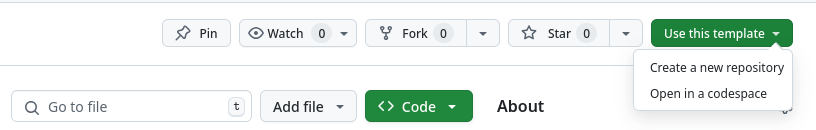
\includegraphics[width=\textwidth,alt={}]{img/template-use.png}
\end{frame}

Pro využití šablon na Githubu klikněte na tlačítko
\enquote{Use this template} na stránce GitHub repozitáře s podporou šablon. 

Tím se ve vašem účtu vytvoří
nový repozitář se stejnou strukturou a soubory. Poté jej můžete naklonovat,
upravit obsah a začít vytvářet vlastní snímky a handouty.

\begin{frame}[fragile]{Vytvoření nového GitHub repozitáře}
  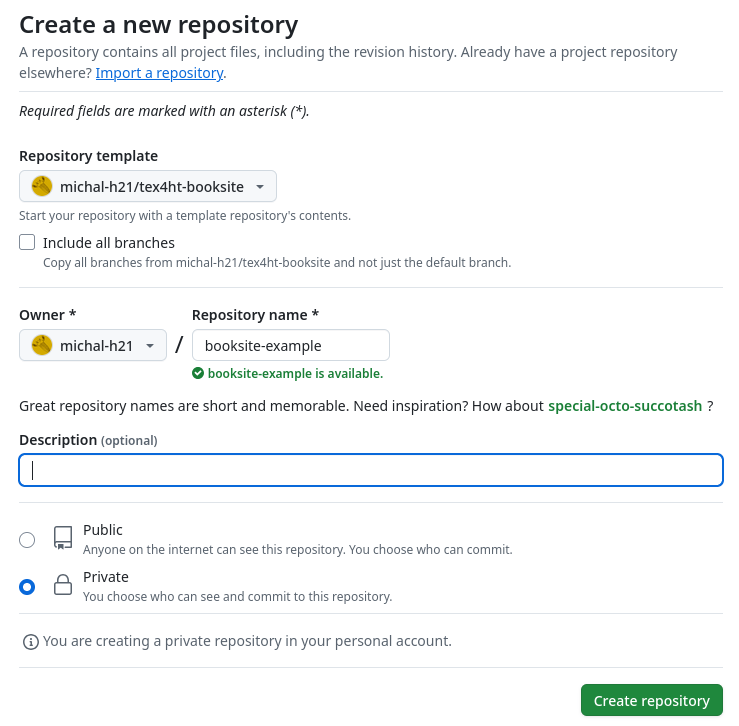
\includegraphics[width=0.6\textwidth,alt={Dialog vytvoření nového repozitáře ze šablony}]{img/new-repo.png}
\end{frame}

Po 

% \subsection{Github Actions}

\begin{frame}[fragile]{Rozhraní Github Actions}
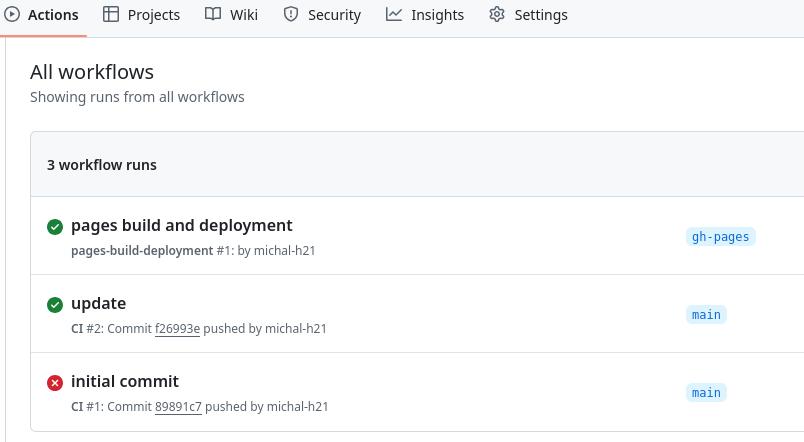
\includegraphics[width=\textwidth]{img/github-actions.png}
\end{frame}

Po pushnutí změn do větve \texttt{main} můžete zkontrolovat záložku
\texttt{Actions} ve vašem Github repozitáři. Zobrazuje stav workflow, včetně
informace o úspěšném dokončení nebo případných chybách.

\begin{frame}[fragile]{Chyby}
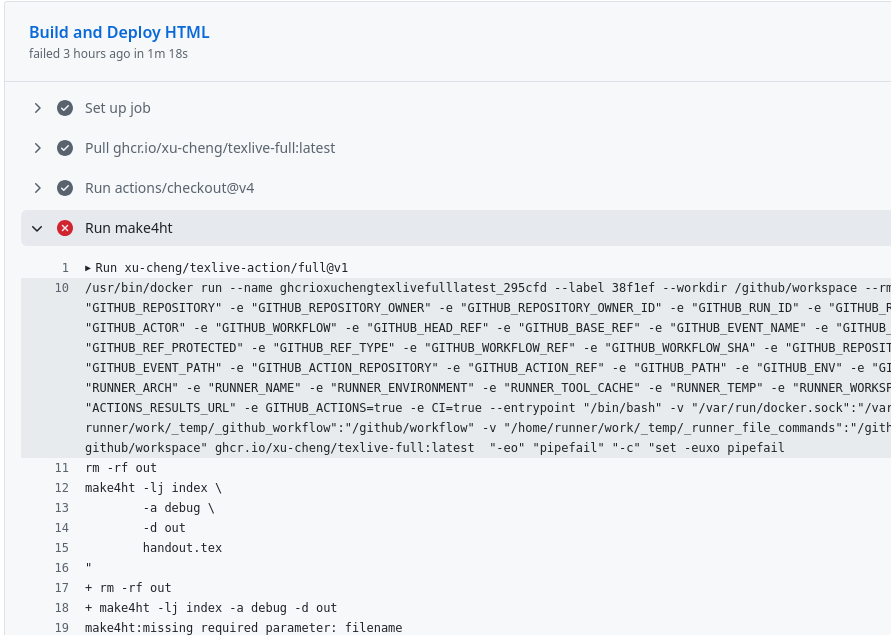
\includegraphics[width=\textwidth]{img/github-error.png}
\end{frame}

Můžete také zkontrolovat logy běhu workflow, abyste viděli, co se pokazilo.
Pokud narazíte na chybu, bude zobrazena v logu a můžete tyto informace
použít k řešení problému.

V tomto případě byl nesprávný název TeX souboru. Musel jsem opravit název
souboru v YAML souboru GitHub Actions.

% \subsection{Publikování HTML verze}

\begin{frame}[fragile]{Nastavení Github Pages}
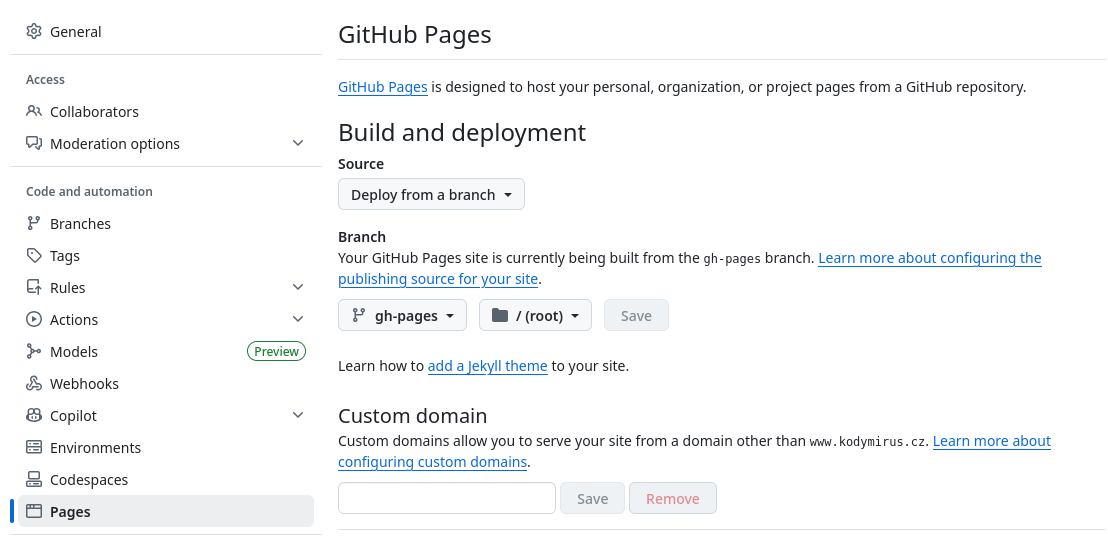
\includegraphics[width=\textwidth]{img/github-pages.png}
\end{frame}

Po úspěšném dokončení workflow můžete nastavit GitHub Pages pro zobrazování obsahu větve \texttt{gh-pages}.

Všechny výstupní soubory vytvořené pomocí \texttt{make4ht} budou dostupné na webu.
Budou přístupné na adrese:
\verb|https://username.github.io/repo/|,
kde \texttt{username} je vaše GitHub uživatelské jméno a \texttt{repo} je název vašeho repozitáře.

Například příklady použité v této prezentaci naleznete na adresách \url{https://michal-h21.github.io/tex4ht-presentation/},
\url{https://michal-h21.github.io/tex4ht-booksite/}

\section{Šablona pro prezentace}

Tato šablona je určena pro prezentace, které potřebují víc než jen snímky. Umožňuje vytvořit jak samotnou prezentaci, tak podrobný handout s poznámkami a komentáři. Všechny materiály tak lze generovat z jednoho zdrojového souboru – jak pro živou prezentaci, tak pro lidi, kteří se prezentace neúčastnili.

Obsahuje několik hlavních zdrojových souborů, každý s konkrétním účelem:

\begin{frame}[fragile]{Přehled souborů}
\begin{itemize}
\item \textbf{\texttt{slides.tex}}
\item \textbf{\texttt{handout.tex}}
\item \textbf{\texttt{presentation.tex}}
\item \textbf{\texttt{preamble.tex}}
\item \textbf{\texttt{config.cfg}}
\end{itemize}
\end{frame}

\begin{itemize}
\item \textbf{\texttt{slides.tex}} – Tento soubor slouží ke generování hlavní prezentace ve formátu Beamer. Obsahuje to, co se zobrazuje během přednášky.

\item \textbf{\texttt{handout.tex}} – Handoutová verze prezentace, formátovaná jako standardní článek. Kromě obsahu viditelného na snímcích obsahuje i doplňující poznámky a komentáře, které se v samotné prezentaci nezobrazují. Tento soubor je určen ke sdílení po skončení prezentace a měl by být samostatně použitelný i pro čtenáře, kteří prezentaci neviděli.

\item \textbf{\texttt{presentation.tex}} – Obsahuje celý zdrojový text prezentace. Obsah uvnitř prostředí \verb|\begin{frame}...\end{frame}| se zahrnuje jak do \texttt{slides.tex}, tak do \texttt{handout.tex}. Text mimo prostředí frame se v prezentaci nezobrazí, ale je součástí handoutu. To umožňuje doplnit prezentaci o podrobnější komentáře, vysvětlení nebo poznámky.

\item \textbf{preamble.tex} – Obsahuje balíčky a definice příkazů používané v prezentaci.

\item \textbf{config.cfg} – Konfigurační soubor pro \TeX4ht. Například zde můžete upravit CSS styly použité ve webové verzi dokumentu nebo redefinice \LaTeX{}ových příkazů.
\end{itemize}

Tyto soubory si můžete upravit podle svých potřeb. Minimálně je vhodné nahradit obsah \texttt{presentation.tex} vlastním textem a případně upravit \texttt{preamble.tex}, pokud potřebujete přidat další balíčky nebo příkazy.

\subsection{Základní použití}


\begin{frame}[fragile]{Použití prostředí frame a komentáře v handoutu}

\begin{block}{}
Základní syntaxe dokumentu používaného v souboru \verb|presentation.tex| vypadá následovně:
\end{block}

\begin{likeverbatim}\verb|\begin{frame}{Název snímku}|\
\verb|obsah snímku...|\
\verb|\end|\verb|{frame}|\
\vspace{1em}
\verb|Komentář, který bude zahrnut pouze v handoutu|
\end{likeverbatim}

\end{frame}

Například zdrojový kód jednoho z předchozích snímků vypadá takto:

\verb|\begin|\verb|{frame}[fragile]{Přehled souborů}|
\begin{verbatim}
\begin{itemize}
\item \textbf{\texttt{slides.tex}}
\item \textbf{\texttt{handout.tex}}
\item \textbf{\texttt{presentation.tex}}
\item \textbf{\texttt{preamble.tex}}
\end{itemize}
\end{verbatim}
\verb|\end|\verb|{frame}|

\begin{verbatim}
\begin{itemize}
\item \textbf{\texttt{slides.tex}} – Tento soubor slouží ke generování hlavní
prezentace ve formátu Beamer. Obsahuje to, co se zobrazuje během přednášky.
\end{itemize}
\end{verbatim}

Obsah uvnitř bloku \verb|\begin|\verb|{frame}...\end|\verb|{frame}| se zahrne
do prezentace i handoutu, ale prostředí \texttt{itemize}, které následuje za
ním, se zobrazí pouze v handoutu.

\begin{frame}[fragile]{Sdílený obsah mimo prostředí frame}

\begin{verbatim}
\mode<beamer|article>{
\title{Strukturovaná šablona prezentace}
\author{Michal Hoftich}
\maketitle
}
\end{verbatim}
\end{frame}

Příkaz \verb+\mode<beamer|article>{...}+ umožňuje zahrnout obsah, který se má
zobrazit jak v prezentaci, tak v handoutu. To se může hodit například pro název
prezentace nebo obsah prezentace.

\subsection{Kompilace prezentace}

\begin{frame}[fragile]{Kompilace do PDF}

Prezentaci nebo handout můžete zkompilovat do PDF pomocí LuaLaTeXu těmito příkazy:

\begin{verbatim}
$ lualatex slides.tex
$ lualatex handout.tex
\end{verbatim}
\end{frame}



Výstupní soubory můžete kompilovat v libovolné standardní distribuci \LaTeX{}u, která obsahuje Beamer a potřebné balíčky.

\begin{frame}[fragile]{HTML verze}
Pro převod prezentace do formátu HTML použijte nástroj \href{https://www.tug.org/tex4ht/}{\TeX4ht}.
\begin{verbatim}
$ make4ht -l handout.tex\end{verbatim}

Přepínač \verb|-l| zajistí použití Lua\LaTeX{}u jako překladače.
\end{frame}

HTML verze se generuje z handoutu ve stylu článku, nikoliv z Beamer prezentace.
To ji činí vhodnější pro webové publikování nebo dlouhodobé sdílení, protože
obsahuje všechny vysvětlivky a není závislá na rozvržení snímků.

section{Automatické generování HTML výstupu}

Tato část vysvětluje, jak se používají \href{https://docs.github.com/en/actions/writing-workflows/quickstart}{GitHub Actions} k automatickému generování a publikování HTML verze materiálů při každém pushnutí změn do větve \texttt{main}.

Výstup je vytvářen pomocí \texttt{make4ht} a publikován do větve \texttt{gh-pages}, což usnadňuje sdílení webové verze prezentace.

\begin{frame}[fragile]{Přehled GitHub Actions}
Klíčové části workflow pro sestavení a publikování HTML:

\begin{verbatim}

    name: Spuštění make4ht
    uses: xu-cheng/texlive-action/full@v1
    with:
      run: |
      make4ht -lj index -a debug -d out handout.tex

    name: Publikování webových stránek
    uses: peaceiris/actions-gh-pages@v3
    with:
      github_token: ${{ secrets.GITHUB_TOKEN }}
      publish_dir: ./out
\end{verbatim}

\end{frame}

Workflow je definován v souboru \texttt{.github/workflows/main.yml}.
Tento soubor můžete upravit pro přizpůsobení procesu sestavení, například změnou parametrů pro \texttt{make4ht}.

Používají se dvě GitHub Actions: \href{https://github.com/xu-cheng/texlive-action}{xu-cheng/texlive-action}
a \href{https://github.com/peaceiris/actions-gh-pages}{peaceiris/actions-gh-pages}.
První umožňuje používat libovolný příkaz dostupný v TeX Live instalaci, jako \texttt{make4ht} nebo \texttt{lualatex}.
Druhá publikuje obsah zadaného adresáře do větve \texttt{gh-pages} vašeho repozitáře,
kterou GitHub Pages používá pro zobrazování statického obsahu.

\begin{frame}[fragile]{Automatické sestavení HTML}
Změny pushnuté do větve \texttt{main} spustí GitHub Actions workflow, který:

\begin{itemize}
\item Zkompiluje \texttt{handout.tex} do HTML pomocí \texttt{make4ht}
\item Publikuje výstup do větve \texttt{gh-pages}
\end{itemize}

Použitý příkaz je:

\begin{verbatim}
make4ht -lj index -a debug -d out handout.tex
\end{verbatim}
\end{frame}

Tento příkaz vytvoří HTML soubory v adresáři \texttt{out/}, které jsou následně publikovány
pomocí akce \texttt{peaceiris/actions-gh-pages}, specifikované nastavením
\texttt{publish_dir}.

\begin{frame}[fragile]{Proč \texttt{-j index}?}
\begin{itemize}
\item Volba \texttt{-lj index} je zkratka pro \texttt{-l -j index}
\item Volba \texttt{-j index} nastaví název výstupního HTML souboru na \texttt{index.html}
\item To umožňuje používat čisté URL adresy jako:

\begin{verbatim}
https://username.github.io/repo/
\end{verbatim}

\end{itemize}
\end{frame}

Není potřeba v URL specifikovat název souboru - GitHub Pages
automaticky hledá soubor \texttt{index.html}. Toto usnadňuje sdílení
prezentace a pomáhá předejít nefunkčním odkazům kvůli neshodě názvů souborů.



\end{document}
\end{verbatim}

\end{frame}


V handoutu můžeme pouít libovolnou třídu dokumentu spolu s balíčkem \texttt{beamerarticle}.
Text prezentace můžeme vložit pomocí příkazu \verb|\input|. 

\begin{frame}[fragile]{Soubor \texttt{preamble.tex}}
\begin{verbatim}
\usepackage{hyperref}
\usepackage{graphicx}
\usepackage[czech]{babel}
...
+ další balíčky a vlastní příkazy
\end{verbatim}
\end{frame}


\begin{frame}[fragile]{Použití prostředí frame a komentáře v handoutu}

  \begin{block}{Základní syntaxe dokumentu používaného v souboru \texttt{presentation.tex}:}
\begin{likeverbatim}\verb|\begin{frame}{Název snímku}|\\
\verb|obsah snímku...|\\
\verb|\end|\verb|{frame}|\\
\vspace{1em}
\verb|Komentář, který bude zahrnut pouze v handoutu|
\end{likeverbatim}
\end{block}

\end{frame}

Například zdrojový kód jednoho z předchozích snímků vypadá takto:

\verb|\begin|\verb|{frame}[fragile]{Přehled souborů}|
\begin{verbatim}
\begin{itemize}
\item \textbf{\texttt{slides.tex}}
\item \textbf{\texttt{handout.tex}}
\item \textbf{\texttt{presentation.tex}}
\item \textbf{\texttt{preamble.tex}}
\end{itemize}
\end{verbatim}
\verb|\end|\verb|{frame}|

\begin{verbatim}
\begin{itemize}
\item \textbf{\texttt{slides.tex}} – Tento soubor slouží ke generování hlavní
prezentace ve formátu Beamer. Obsahuje to, co se zobrazuje během přednášky.
\end{itemize}
\end{verbatim}

Obsah uvnitř bloku \verb|\begin|\verb|{frame}...\end|\verb|{frame}| se zahrne
do prezentace i handoutu, ale prostředí \texttt{itemize}, které následuje za
ním, se zobrazí pouze v handoutu.

\begin{frame}[fragile]{Sdílený obsah mimo prostředí frame}

\begin{verbatim}
\mode<beamer|article>{
\title{Strukturovaná šablona prezentace}
\author{Michal Hoftich}
\maketitle
}
\end{verbatim}
\end{frame}

Příkaz \verb|\|\verb+mode<beamer|article>{...}+ umožňuje zahrnout obsah, který se má
zobrazit jak v prezentaci, tak v handoutu. To se může hodit například pro název
nebo obsah prezentace.

\section{Závěr}

\begin{frame}[standout]{}
  \begin{block}{}
    Děkuji za pozornost!
  \end{block}
  \begin{block}{}
    \small
  \url{https://www.kodymirus.cz/presentations/ossconf2025.html}
  \end{block}

\end{frame}





